\chapter{Setting the scene}\label{ch:theory}
\section{Introduction}
This chapter provides an outline of the theoretical discussion on verb serialisation, picking up the thread from the introductory chapter where I roughly characterised serial verbs as `underspecified' verb sequences. Reviewing the properties that have been proposed to characterise these strings, I will in this chapter arrive at a revised definition of what to count as such. The last decades have witnessed a sharp increase in studies into verb serialisation, both from a descriptive point of view as well as from theoretical and typological perspectives. The body of literature is so vast that it is beyond the scope of this chapter to fully review and discuss it. I will rather concentrate on some of the most influential contributions and single out the main arguments and features.

The chapter consists of four parts. The first part aims at giving a general overview of the literature. It is here that basic concepts such as monoclausality or argument sharing are introduced. As we proceed, we will see that there are both criteria that are used to delimit serialising constructions from other construction types, as well as criteria that are assumed to account for SVC-internal variation (giving rise to much controversy as to which properties SVCs need to have, and which might be optional or dependent upon areal convergence). 

From the close examination of these different criteria I will then, in the next part, turn to work that has been carried out either within the area of Eastern Indonesia or in adjacent regions on related languages. Specifically, I will review Bril's work on SVCs in Oceanic languages \citep{bril2004complex,bril2007nexus}, Pawley's and Lane's work on SVCs in Kalam (the most well-known serialisation system in a Papuan language; \citealt{Pawley1987, pawley2011event, lane2008kalam}), and finally have a closer look at the areal account of SVCs in East Nusantara by \citet{vanstaden2008serial}. The purpose of this section is to review the different classificatory systems in order to test whether they qualify for the study of multi-verb strings in Eastern Indonesia. While I will in this book make use of the more neutral term \textsc{multi-verb construction} (see §\ref{sec:defining} below), the literature survey will help identify important parameters that may be applied cross-linguistically in order to shed light on covert, or at least inconspicuous, differences in the make-up of MVCs across different languages.

In part three, I will introduce the concept of multi-verb construction as an alternative to the serialisation idea. The use of the term multi-verb construction is far less widespread than the SVC concept and its definition is not yet settled. It is, I argue, therefore less laden with presumptions and theoretical restrictions, and better suited to an explorative analysis of multi-verb patterns in EI. 

The final part of this chapter turns to more practical issues and presents an overview of how I evaluated the data sources and which decisions I made concerning the identification of verb sequences. 

\section{Properties of serial verb constructions} \label{section:properties}

In descriptions of serial verbs it is common to start the discussion by giving some justification that the structures in question are indeed serial verb constructions. This is done so typically not by giving a language-specific definition but by listing a set of crosslinguistically valid properties or characteristics. These key characteristics are widely distributed across both descriptive and typological work, and are sometimes assumed to be true without really putting them to the test. 

\subsection{Key characteristics} \label{subsection:keychars}

The `standard list' of properties seems to include at least the following items:

\begin{itemize}
\item SVCs are monoclausal
\item SVCs share at least one argument
\item SVCs have the intonational properties of a single clause
\item SVCs are conceptualised as a single event
\end{itemize}

Some points that follow from this are obvious. First and foremost, although verb serialisation is a phenomenon that apparently originates in syntax (a series of verbs crosscutting the traditional clause-linking strategies), most characteristics are drawn from other linguistic areas, for example from prosody or from cognition. Only the first characteristic, monoclausality, seems to spring directly from syntax. The problem with monoclausality is that definitions of `clause' tend not to be universally applicable so that we end up in a situation where we try to define SVCs by putative universal characteristics that in turn depend upon language-specific features. \citet[298]{haspelmath2016serial} notes that \begin{quote}[s]yntacticians often distinguish between monoclausal and biclausal constructions, and there is a voluminous literature on clause fusion, i.e. synchronic or diachronic derivation of a monoclausal pattern from a biclausal pattern
(restructuring, clause union, coherent infinitives, etc.). However, the criteria for determining clausehood are generally language-specific.\end{quote}

Other parameters are equally problematic: the prosody paramater is sometimes given as `homogeneous intonation contour' (whatever syntactic constituent might be found underneath), and sometimes the argument also invokes the clause concept (`monoclausal prosody'), assuming that there is a definable prosodic unit that is always and invariably tied to the clause). While the former phrasing presupposes a clear concept of an intonational phrase in that particular language, the latter presupposes both a clearly defined IP, and a clause. Similar problems arise with the `single event' notion.

Maybe it is for this reason that the standard list of defining characteristics has been elaborated by many authors time and again, with the addition of further properties from different linguistic layers. Table \ref{tab:keyfeatsvc} below presents a list of properties that have been proposed quite frequently, including the standard ones given above. It is certainly not exhaustive, but may suffice to delimit the field of the more prominent SVC definitions.

\begin{table}\small
\begin{tabularx}{\textwidth}{QQQ}
\lsptoprule 
Parameter & Test & Literature \\
\midrule \multicolumn{3}{c}{Lexical level}\\\midrule  
  independent verb(s) & construe verbs as simplex predicate & \citet{bril2004complex, Aikhenvald2006, haspelmath2016serial} \\
\midrule \multicolumn{3}{c}{Grammatical level}\\\midrule
  no junctor & insert junctor & \citet{Aikhenvald2006, muysken2006serial, haspelmath2016serial} \\
  monoclausality & apply clause defining operations, relativisation, apply negator & \citet{bril2004complex, Aikhenvald2006, haspelmath2016serial} \\
  no dependency & observe/apply verb morphology & \citet{Durie1997, Aikhenvald2006} \\
  single subject/ external argument & insert different subject referents & \citet{Durie1997, muysken2006serial} \\
  shared argument(s) & insert different argument referents & \citet{Durie1997, bril2004complex}, \citep{Aikhenvald2006} \\
  single predicate/ predication & apply predicate defining operations & \citet{bril2004complex, Aikhenvald2006} \\
  shared operator value & apply different operators & \citet{Durie1997, bril2004complex, Aikhenvald2006, muysken2006serial} \\
\midrule \multicolumn{3}{c}{Prosodic level}\\\midrule
  single pitch contour & check IU defining properties & \citet{Durie1997, bril2004complex, Aikhenvald2006} \\
  no internal pauses & measure speech flow (interuptions) between verbs & \citet{bril2004complex, muysken2006serial} \\
\midrule \multicolumn{3}{c}{Cognitive level}\\\midrule
  single event & apply event defining operations, MEP & \citet{Durie1997, Aikhenvald2006} \\
\lspbottomrule
\end{tabularx}
\caption[Key characteristics of SVCs]{Prominent key characteristics of SVCs and their occurrence in selected publications. Citations in brackets mean that the feature is not regarded as obligatory by the author. Note that the tests are inferred from the literature, and not necessarily proposed or used that way by the specific authors.} \label{tab:keyfeatsvc}
\end{table}

As already indicated, there are basically two types of parameter: parameters of the first type can be assessed directly by applying some straightforward operation. For instance, the parameter `no junctor' may be put to the test simply by trying to add one. Or the independence of a verb may be tested just by putting it into predicate function, i.e., creating a monoverbal predicate. The results of these operations are not always straightforward but at least there is a clear testing procedure available. 

The second type of parameter, on the other hand, relies upon further features that need to be tested beforehand. This is exactly the monoclausality problem from above. I call this type a dependent parameter because it relies on further information that often need to be gathered from the language in question (i.e., there is no crosslinguistically valid procedure). Examples of this type of parameter all have the test description `apply X defining operations' in Table \ref{tab:keyfeatsvc}. It is these parameters that are most prone to circularity. For example, it is tempting to argue that SVCs only consist of one predicate by resorting to quite unrelated concepts such as clausehood or syntactic dependency, as the following discussion in \citet[4]{Aikhenvald2006} under the header `Serial verb construction as a single predicate' illustrates:
\begin{quote}An SVC functions on a par with monoverbal clauses in discourse... act together as a syntactic whole... [is] often translatable as single predicates into non-serializing languages... cannot take separate markers of syntactic dependency.\end{quote} 

Instead of directly assessing the predicate status Aikhenvald resorts to a range of concomitant feature values such as lack of dependency markers or syntactic unity. The problem of circularity in these arguments is long known. Givón, for instance, has called the single clause/single event arguments ``a problematic straw man" \citep[84]{givon1991serial}. He continues by stating that
\begin{quote}[o]n the structural side, `single clause' is a notion that retains a high potential for circularity. One can
easily define `clause' as a construction with a single verb at its core. On the cognitive side, `single event' is just as susceptible to the very same circular definition, and linguists are notoriously prone to letting grammatical structure define what is a `single event'.\end{quote}

Another circular argument in favour of the monoclausality parameter is also quite common: The evidence that a SVC is monoclausal is often drawn from the fact that it has a ``monoclausal intonation contour". This can of course easily be flipped into the argument that SVCs have a coherent intonation contour just because they consist of a single clause. This way of cycling between the concepts leads to a situation that is crosslinguistically hard, if at all, accessible. As \citet[299]{haspelmath2016serial} points out, 
\begin{quote}[f]rom the current perspective, this is fatal: Comparative concepts must be defined in such a way that the definition is equally applicable to all languages. Applying different diagnostics to pick out the same phenomenon in different languages would make sense only on the view that a notion such as ``clause" is an innate category of universal grammar.\end{quote}

In the following sections, I will have a closer look at the different parameters from Table \ref{tab:keyfeatsvc} and discuss the arguments that have been raised in their favour.

\subsubsection{Lexical properties}\label{sec:lexprop}

The most influential parameter on the verb level is the independent verbs parameter suggesting that each verb in a SVC should in principle be able to occur on its own (behaving like a full-fledged independent verb). The first question that arises here is whether verbs are in fact always independent in this sense. Or are there also verbs that are not independent but may only occur in combination with some other item (which then is probably another verb or something quite related)? There are many examples of items that seem verb-like in one regard and yet cannot occur as an independent verb. For instance, auxiliaries or modal verbs show verbal properties in many languages (for instance, they may inflect or occupy the main verb slot in a clause). Another class of verb-like items is the coverb class that pervades the grammar of many Australian languages. Here it is their capacity to provide the argument frame that makes them look quite verbal (although what takes the inflection is a generic verb). Basically because coverbs do not inflect for verbal categories, Schultze-Berndt argues for Jaminjung that coverbs form a distinct lexical category \citep[71]{schultze2000simple}. The `real' verbs, on the other hand, are comprised of a smallish class of about 30 members and possess quite generic meanings although simplex predicates with just one of these generic verbs constitute about 40\% of verbal predicates in texts \citep[118]{schultze2000simple}. The fact that many event concepts in languages such as Jaminjung can only be expressed by combinations of a coverb and a generic verb (`complex predicates') still suggests that coverbs may qualify as verbs (though not as prototypical ones).

So, the answer to the question: are there verbs that are not independent? is, frankly, yes. There are lexemes that show verb-like behaviour and yet do not fulfill all requirements of verbs in that particular language. Now, on which ground may we qualify or disqualify them as possible hosts in SVCs? Authors that discuss the `independent verb' parameter seem to assume that multi-verb strings with such verbs do not constitute SVCs because SVCs are viewed as ephemeral combinations of free verbs occurring on the spot without any dependency relations. For instance, \citet[303]{haspelmath2016serial} gives the following definition: \begin{quote}comparative concept `independent verb’:

for comparative purposes, an independent verb is a form that can express a dynamic event without any special coding in predication function and that can occur in a non-elliptical utterance without another verb.\end{quote}

Two things are of crucial importance in Haspelmath's definition: first, independent verbs express dynamic events. This is interesting because it is (to my knowledge) the first attempt to disqualify SVCs with stative verbs altogether. \citet[302]{haspelmath2016serial} argues that \begin{quote}the only workable criterion for noun, verb and adjective as comparative concepts is the use of an item in a particular information-packaging function without special coding such as a copula. Thus, verbs are defined as dynamic event expressions that do not have special coding when used in predication function.\end{quote}

The second crucial parameter in Haspelmath's definition is the `non-elliptical utterance'. Ellipsis is a well-known problem in SVC analysis because elliptical utterances may be mistaken for full-fledged constructions. Consider for illustration the following stretch of Wooi narrative:


\ea 
\langinfo{Wooi}{Austronesian, SHWNG}{traditional\_land\_Kirihio1\_exp 27-29}\\
\ea
\glll Rakuar hembepinda rea \\
Rakuar he-ve-pinda rea \\
Rakuar \textsc{3}\textsc{pl}-\textsc{vblz}-move again \\
\glft `The Rakuar people moved again,' \\ 
\ex \label{wooi-kong}
\glll hengkong hnia na riumpey \\
he-kong hnia na riung-pey \\
\textsc{3}\textsc{pl}-with \textsc{3}\textsc{pl} \textsc{loc} top-\textsc{upward} \\
\glft `they (stayed) with them up there,' \\ 
\ex
\glll hena kuyra na Hopi mariayng vane \\ 
he-na kikuyra na Hopi maria-ayng vane \\
\textsc{3}\textsc{pl}-stay together \textsc{loc} Hopi river-bottom \textsc{det}.\textsc{nprx} \\
\glft `they stayed together at the estuary of Hopi river.'\\ 
\z
\z

If we have a look at the second clause, we encounter a verb that is glossed like a preposition (or a preposition that behaves like a verb). In fact \textit{kong} in Wooi is one of these in-between items that have been called prepositional verb in other languages (for instance, by \citet{dol2007grammar} in her grammar of Maybrat). \textit{Kong} in Wooi does not typically take a person indexer when it is used as a postverbal preposition in the sense `do sth. (together) with X' where X denotes a person or a group of people. However, in certain contexts it does inflect and sometimes it occurs on its own, as in example (\ref{wooi-kong}) above. What is interesting here is that our native language specialist added a verb to his Indonesian translation (\textit{mereka (tinggal) dengan mereka di atas}), as if he felt the need to furnish the clause with a `proper' verb (imitated in the English translation by adding the verb `stay'). In constellations such as this one, one could arguably analyse the clause as consisting of an elliptical construction with underlying \textit{hena hengkong} although this would still leave the question why \textit{kong} is marked with the person indexer here. Such data pose serious problems for the question whether (i) a given item is a verb, and (ii) a given item is in fact able to act independently. For the purpose of this study, I excluded all those cases from the dataset for which I could not gather evidence that the verbal item in question may also be used as a simplex predicate. Though not every verb has been put to the test, doubtful lexemes such as Wooi \textit{kong} were searched for in other parts of the published data source, and consequently dismissed if no further data points could be found. An exception to this procedure was made with lexemes that had modal or auxiliary verb semantics. These were counted as 'verboid' and assumed to be verbal (but not fully so, as their rather abstract semantics would normally prevent a simple predication). The same goes for verb-like items that by virtue of grammatical restrictions are to co-occur with other verbs (as, for instance, the group of post-verbal modifier verbs in Wooi; see §\ref{sec:identifyingverbs} for a brief discussion).

Modal verbs and their kin are indeed crucial to the discussion of independent verbhood. For instance, by defining `verb' as given above Haspelmath tries to exclude examples like English \textit{will go} where the bare auxiliary occurs for instance in elliptical answer formulae such as \textit{Yes, I will}. Other verblike elements that would be excluded on these grounds are for instance role-marking verbs in some languages (for instance `accompany/with' or `benefit/for'). 

Another problem with lexical approaches is polysemy between verbs that occur on their own and the `same' verbs occurring in a SVC. \citet{enfield2009review} in his review of Dixon and Aikhenvald's edited volume on SVCs compared such verb pairs from the descriptive chapters and found that authors handle polysemous verbs quite differently. While some authors are rather liberal and allow verbs to be semantically related, other authors exclude ``mere relatedness between an item in the two contexts" \citep[448]{enfield2009review}. He concludes that ``[o]pinions will differ as to whether two lexical entries with different but related meanings should be considered `the same verb’".

Summarising the points, the notion of `independent verb' seeks to exclude certain classes of elements that exhibit verbal properties. In a certain way, this is problematic since verb serialisation as a concept makes use of the notion `verb', and verbs are often not explicitly defined as independent predicators. The question `what is a verb in language x' may then yield a quite different answer from the question `what is an independent verb in construction Y'. As \citet[304]{haspelmath2016serial} concedes, ``[f]rom a language-specific point of view, it may of course still be useful to include these cases [i.e., non-independent verbs, V.U.], e.g. because they may take aspect marking". A further point that remains unclear is how to deal with semantic alternation between verbal items in simplex predicates as opposed to multi-verb predicates. A strict monosemy approach would demand the exclusion of any verbal item that shows contextual deviation in its semantic components.

\subsubsection{Grammatical properties}\label{sec:gramprop}

Under grammatical properties (in a rather loose sense) we can group seven identificational criteria of SVCs: (i) monoclausality, (ii) no dependency, (iii) single subject/external argument, (iv) shared arguments, (v) single predicate/predication, (vi) shared operator value, and (vii) no junctor.

\textsc{monoclausality}. I have already commented on the difficulties of this argument above. It hinges on how clauses are defined. As \citet[26]{lane2008kalam} remarks, to make such an argument presupposes that `the clause' exists both as a single notion on which all linguistis can agree, and as a linguistic unit that is clearcut and identifiable across all languages. While typical clauses with one inflected verb are uncontroversial, multi-verbal clauses may exhibit quite different degrees of compactness of construal. One candidate for clause identification is the classical head as defined by finiteness morphology on the main verb (see also section §\ref{sec:headedness} on headedness in the next chapter). As there are many examples of SVCs with two or more inflected verbs in sequence, this approach would raise the question whether all inflected verbs are indeed heads or whether we may speak of cases of inflection copying or spread. Most SVC languages exhibit the pattern that if verbs are inflected, it is minimally V$_1$ that carries inflection marks. Cases with V$_{\textsc{fin}}$ inflection seem to be much rarer even in verb-final languages. This result is also found in the EI languages (see §\ref{sec:headedness}).

A second diagnostic for clausehood is the scope behaviour of operators. Such approaches have become especially popular within Role-and-Reference Grammar's (RRG) layered structure of the clause. The claim is that different operators target different clausal layers \citep{foley1984functional}. While aspect and directionals are connected to the nucleus, other operators such as tense target the peripheral layer of the clause, i.e., are indicative of the outer boundaries of the clause. \citet{haspelmath2016serial} argues in a similar way for a crosslinguistic clause diagnosis, following \citet{bohnemeyer2007principles}, who observed the behaviour of negators within clauses. Negation as an indicator for monoclausality can be used in at least two different ways. First, one could argue that the scope of the negator has to stay the same. Different authors take different positions in this regard. Examples like the following one from Alamblak (Papua) illustrate that in some languages there are different possible interpretations available. The utterances from (\ref{ala-1}) to (\ref{ala-2}) are all possible replies to the negated serial verb construction, differing in the way the scope of the negator is understood.

\ea 
\langinfo{Alamblak}{Papuan, Sepik}{\citealt[27]{bruce1988}}
\ea \label{alamblak1}
\gll ritm fiñnji tandhi-ak-ni-r-më-t-m \\
insects \textsc{neg} roast-get-go-\textsc{irr}-\textsc{rem}.\textsc{pst}-\textsc{3}\textsc{sg}.\textsc{f}-\textsc{3}\textsc{pl} \\
\glft `She did not roast (and) get the insects (and) go.' \\ 
\ex \label{ala-1}
\gll nɨfrim haynimëtm \\
uncooked she:took:them \\
\glft (negative on `roast') \\ 
\ex
\gll tandhihɨtatañhatë \\
having:roasted:(and):left:(them) she:went \\
\glft (negative on `get') \\ 
\ex
\gll yohre tandhiyakitëhhasiwtm \\
still she:is:roasting:(and):holding:them \\
\glft (negative on `go') \\ 
\ex
\gll nɨfrim hɨtatañhatë yimët \\
uncooked \textsc{sa}:having:left:(them) she:went \\
\glft (negative on `roast' and `get') \\ 
\ex
\gll tandhihatë ruhhasëmët \\
\textsc{sa}:having:roasted:them she:was:remaining \\
\glft (negative on `get' and `go') \\ 
\ex \label{ala-2}
\gll yohre tandhitwëtm \\ 
still she:is:roasting:them \\
\glft (negative on all three roots)\\ 
\z
\z

\citet{Aikhenvald2006} proposed that ``[t]here can only be one negator per SVC. It can either have the whole construction as its scope [...] or part of the construction." Under this view, the Alamblak case in (\ref{alamblak1}) to (\ref{ala-2}) above would be fine. \citet[293]{Durie1997}, on the other hand, seems to take another stance and defines SVCs as having ``shared tense, aspect, mood and polarity: this is often reflected in a single morphological realization of these operators [...], or in obligatory concord across the verbs [...]." SVC constructions in Paamese, he argues, lose their SVC interpretation as soon as the scope of the negator is over the second verb constituent alone.

A second way to operationalise negator behaviour is by looking at their construal. This is what \citet{haspelmath2016serial} and  \citet{bohnemeyer2007principles} suggest: within one clause, there should be only one negation pattern. That is, if the negator is placed with the second verb, the same construction should not be possible with the negator being placed with the first verb \citep{haspelmath2016serial}. The Alamblak case in (\ref{alamblak1}) to (\ref{ala-2}) would under this view be a well-formed SVC as the negator placement remains constant across all scope variations.

A final interesting piece of evidence for clausehood and clause boundaries comes from the behaviour of reflexive binding. We know from generative research into binding that reflexive pronouns may only be bound within its governing category, i.e., the clause. Reflexive pronouns could thus be a measure of clause boundaries in SVCs. Consider the following example from Saramaccan, a creole language from Suriname:

\ea \label{}
\langinfo{Saramaccan}{Creole, English based}{\citealt[299]{muysken2006serial}}\\
\gll di mujee$_i$ da di pikin$_j$ di sopi wasi en-seei$_{*i/j}$ \\
the woman give the child the soap wash \textsc{3}\textsc{sg}-self \\
\glft `The woman gave the child the soap to wash himself (*her) with it.'\\ 
\z

The child is the only argument that can control the reflexive pronoun \textit{enseei}. If the woman \textit{mujee} is the theme of the washing, the independent pronoun \textit{en} would have to be used instead of \textit{enseei}. The construction thus arguably consists of two clauses. Arguments of this sort seem otherwise rare in the literature on serialisation (but see \citealt[514]{baker1989object}) and I have not come across a single example of binding evidence in EI languages. 

In this book, I excluded the monoclausality criterion for both theoretical and practical reasons (see discussion in §\ref{sec:defining} further below).

\textsc{no dependency}. This argument is somewhat less prominent than others but is repeatedly given. Aikhenvald writes: ``Unlike coordinate or subordinate structures, SVCs cannot, by definition, contain any marker of syntactic dependency" \citep[20]{Aikhenvald2006}. Which markers she has in mind remains, however, unsaid. Vague statements like this are also found in descriptive work. For instance, Baird writes about SVCs in Klon: ``We know that verbs within a serial complex are not subordinate to one another, because of their other structural characteristics" \citep[136]{baird2008motion}. \citet[291]{Durie1997} is more explicit on this, saying that ``one verb is not embedded within or as complement of the other". Though Durie does not refer to morphological formatives but to dependency relations as such, it becomes clear that it is instances of verbal complements that are felt to be different from SVCs. Verbs then should not show non-finite or infinite morphology which would indicate complementation or embedding. Also, according to Durie, complementisers and other hierarchising formatives should be absent from SVCs. 

Dependency in its basic sense means that out of two constituents, one dominates the other so that the latter is dependent upon the former. Dependency is at work in different parts of human grammar but for our purpose, the most relevant dependency types are those between verbs and other clausal constituents. Governance is a kind of dependency that holds between a verb and its arguments (see also \citealt{bril2007nexus} on the notion of dependency). If the argument position of a verb is filled by another verb (and its arguments), we get a sentential complement. As structures like \textit{Bill saw that the crocodile was heading towards him} are common in most of the world's languages, most proponents of verb serialisation would argue against lumping complementation together with serialisation. Yet, in many serialising languages, sentential complements look just like other types of SVCs: there is neither dependency marking on the verbs, nor are there overt complementisers. This is why authors like Durie or Haspelmath directly make reference to complements or predicate-argument relations, attempting to keep them out of the group of `proper' SVCs. Haspelmath writes: ``it is better to exclude them, because they do not belong to the original core of SVC phenomena" \citep[15]{haspelmath2016serial}. Aikhenvald, on the other hand, regards ``serialization of verbs of speech [as] a subtype of verb serialization as a complementation strategy" \citep[25]{Aikhenvald2006}.   

\textsc{single subject/external argument}. This criterion demands that there be only one subject/external argument in a SVC. I assume that the reason for this criterion is that if there is only one subject or external argument in the whole construction, then surely we must be dealing with a single clause/single predicate. While it does make good sense with the bulk of SVC types, there is a specific problem with SVCs that obviously encode two different subjects. Consider the Paamese example below:

\ea \label{paamese1}
\langinfo{Paamese}{Austronesian, Oceanic}{\citealt[55]{crowley2002serial}}\\
\glll inau nuas vuas he:mat \\
inau ni-uasi vuasi hee-mate \\
\textsc{1}\textsc{sg} \textsc{1}\textsc{sg}:\textsc{dist}.\textsc{fut}-hit pig \textsc{3}\textsc{sg}:\textsc{dist}.\textsc{fut}-die \\
\glft `I will hit the pig to death.' \\ 
\z

The construction in (\ref{paamese1}) consists of two verbs, each one marked with a subject indexer. The subject indexed on the hit verb, however, does not reappear on the second verb. Instead the object referent of the hitting is reanalysed as subject of the die verb. This has sometimes been addressed as `pivotal constructions' where one argument is assigned two functions. Quite unlike most other types of SVCs, the `switch-function' type does allow this kind of conflicting subject index. Such patterns have led some authors to quite surprising interpretations. \citet[292]{Durie1997} remarks on the same construction in Paamese: \begin{quote}Despite the multiple subject prefixes, there can only be one true subject NP in Paamese core serialization. This appears before V$_1$. An attempt to insert a second full subject NP before the second verb changes the meaning of the sentence to a biclausal interpretation.\end{quote}

Of course, he is right in observing that inserting two NPs between the verbs apparently leads to a different construction. Example (\ref{paamese2}) illustrates what happens when the pivotal argument is split up into two NPs each one bearing one function (being co-referential).

\ea \label{paamese2}
\langinfo{Paamese}{Austronesian, Oceanic}{\citealt[56]{crowley2002serial}}\\
\glll inau nuas vuasi kai he:mat \\
inau ni-uasi vuasi kaie hee-mate \\
\textsc{1}\textsc{sg} \textsc{1}\textsc{sg}:\textsc{dist}.\textsc{fut}-hit pig \textsc{3}\textsc{sg} \textsc{3}\textsc{sg}:\textsc{dist}.\textsc{fut}-die \\
\glft `I will hit the pig and it will die.'\\ 
\z

The first thing we notice is that the construction only changes with regard to the number of argument slots\footnote{One of Crowley's arguments for a biclausal construction is that one can insert the coordinator \textit{kaa} `and' between \textit{vuas} and \textit{kai} \citep[56]{crowley2002serial}}. It is only in the semantics that we find subtle differences. Example (\ref{paamese1}) appears to describe one coherent process of hitting the pig until death occurs. I assume that the \textsc{hit} verb in this sense is understood as happening repeatedly. If the event were to be sliced into small time portions, hitting would probably occur within each portion, and the pig's constitution would progressively suffer with each blow. In (\ref{paamese2}), on the other hand, a biclausal sequential reading is produced, where the hitting seems to be bound in time and only afterwards followed by the death of the pig (which may occur after a delay). 

But what does this mean with regard to the `single subject' claim? If there is only one ``true subject NP" in (\ref{paamese1}) as Durie claims what does the second verb index? If prefixes mark subjects in Paamese we would not probably want to say that in a small number of cases (in one particular construction), the same prefix instead denotes the object of the preceding verb, or should be ignored altogether. Another alternative would be to claim that there are two kinds of subjects in Paamese: `minor' subjects, or whatever one might call them, are crossreferenced on the verbs, as usual; higher level `constructional' subjects, however, do not receive marking but are defined by position of the argument in the construction. Both options are highly unwelcome from both a descriptive and a theoretical perspective, and thus the `single subject' claim seems unattractive when reviewed properly. Contemporary authors now rather speak of single semantic roles in SVCs (for instance \citealt{haspelmath2016serial}), and this would intuitively make more sense for constructions like (\ref{paamese1}) where both \textsc{ego} and the pig occupy very different semantic roles (actor versus undergoer, or, more fine-grained, agent versus patient).

\textsc{shared arguments}. In SVCs, there is typically one, or more than one, argument that is `shared' among the verbs. Sharing implies that both verbs license arguments of which two happen to be co-functional or at least co-referential. \citet{haspelmath2016serial}, while not including this parameter in his definition of SVCs, gives a brief overview of different types of argument-sharing in SVCs. He distinguishes between agent-sharing SVCs and patient-sharing (both with subgroups). Generally, this parameter does not receive much discussion in the literature as it seems to be applicable in a straightforward manner.

If argument-sharing is adopted as a `hard' definitional boundary then some putative SVCs have to be dropped. The most controversial cases are probably `ambient serialization' and cumulative argument SVCs. Ambient serialization involves a modifier verb with a 3SG subject indexer that takes the other VP as its single argument (much like, for instance, \textit{your coming here, it was quick}). Cumulative argument SVCs are formed by a joint group verb like `accompany' and a further verb. The group verb takes a subject and an object argument, both of which are collapsed into a plural subject indexer on the second verb (I follow you, we go-constructions). In both cases, one may argue that no argument is actually `shared' between the verbs. This issue is, like most others, not yet settled, and authors give different verdicts. \citet[12]{Aikhenvald2006} for instance is quite liberal in saying that \begin{quote}[p]rototypical serial verb constructions share at least one argument. Serial verb constructions with no shared arguments are comparatively rare, but not non-existent.\end{quote}
Durie is not quite clear on this point. On the one hand, he demands that ``serial verbs `share' at least one and possibly more arguments" \citep[291]{Durie1997}, while at the same time he happily includes an example of a cumulative argument SVC from Paamese:

\ea \label{}
\langinfo{Paamese}{Austronesian, Oceanic}{\citealt[294]{Durie1997}}\\
\glll makurik lovaha \\
ma-kuri-ko lo-va-haa \\
\textsc{1}\textsc{sg}-\textsc{imm}-take-\textsc{2}\textsc{sg} \textsc{1}\textsc{du}.\textsc{in}-\textsc{imm}-go \\
\glft `I take you away with me.' \\ 
\z

According to Durie's analysis, ``the subject of the second verb subsumes both the subject and the object of the preceding verb" \citep[293]{Durie1997}. While this is probably no more exotic than, say, \textit{you and me, we are friends} would be in English, I would rather call this a sharing of referents than a sharing of arguments as the subject argument of the second clause is grammatically referred to with the 1\textsc{du} marker (and thus is construed independently here).

\textsc{single predicate/predication}. The notion predicate forms part of the traditional core of modern linguistic reasoning and is assumed to have universal applicability on a par with clausehood or intonational phrases. Yet if one looks at contemporary textbooks, one finds that predicate definitions are not as common as would be expected for such a fundamental phenomenon (see also \citealt{baker2010complex}). In Payne's much used guide for field linguists \parencite{payne1997describing}, for instance, verbal predicates are largely absent from discussion. And Kroeger in his \textit{Analyzing Grammar} from 2005 only touches briefly upon the notion in order to introduce the grammatical relations. He writes \citep[53]{kroeger2005analyzing}:
\begin{quote}A statement, then, is a sentence which asserts a proposition, i.e. a claim that a certain state of affairs does or does not exist. Normally statements are made about something or someone; they claim that a certain state of affairs is true of a given individual or set of individuals (where the individual may
be a person, place, thing, etc.). [...] The element of meaning which identifies the property or relationship is called the predicate.\end{quote}
While this seems to be something that undergraduates learn in their first semester, it becomes puzzling as soon as the concept predicate is put to use in a context where there is more than one verb in one (alleged) clause. Predicates (and their predicators) come with a number of arguments and assign grammatical functions to them. As verbs are the most typical predicators in language, each verb may in principle count as one predicate nucleus providing a range of argument slots and assigning a grammatical function to them. There is no reason why this assumption should not hold for verbs in SVCs (which means that SVCs do not automatically defy a multi-predicate analysis).

However, the most common reading of the predicate argument in the serialisation literature suggests that SVCs are multiverbal predicates (that is, monopredicational constructions). \citet{klamer1998grammar} opens her chapter on `complex verbs' in Kambera with the definition that ``[s]erial or multi-verb constructions in Kambera are combinations of two verbs that jointly constitute a single predicate". This view seems indeed most appealing in languages where several verbs recveive a single set of affixes forming what \citet{foley1984functional} have called nuclear layer serialisation (see §\ref{sec:nuclear} below). Consider the following Kambera example:

\ea \label{}
\langinfo{Kambera}{Austronesian, CMP}{\citealt[277]{klamer1998grammar}}\\
\gll na-palài nyara-ha$_k$ [da ahu]$_k$ la mbomang \\
\textsc{3}\textsc{sg}.\textsc{nom}-run chase-\textsc{3}\textsc{sg}.\textsc{acc} \textsc{art} dog \textsc{loc} space\_under\_house \\
\glft `He ran after the dogs under the house.' \\ 
\z

We can see that the affix set marking the subject and the object is distributed over both verbs. As the \textsc{run} verb is intransitive it seems natural that the object marker attaches to the second (the transitive) verb. Yet we also find combinations of two transitive verbs with the same affix distribution showing that the object suffix in this construction has to attach to the second verb and not to the first. Examples like this one create conflicting evidence for predicatehood: on the one hand, there are clearly two verbs involved that each contribute different arguments. On the other hand, the surface structure behaves like there really is only one (complex) verb predicating the proposition.

Further confusion with this argument is produced where predicate is distinguished from predication. Bril defines complex predicates\footnote{This term is already problematic. Judging from what has been included under the term `complex predicate', complex predicates are a related yet not identical phenomenon to verb serialisation. It covers, among others, coverb constructions in Australian languages, periphrastic causative constructions in Romance languages, auxiliary verb constructions in English (\textit{will go}, precisely the \textit{will} that is elsewhere with great effort excluded from serialisation through the `independent verb parameter' from above), and many other constructions that involve generic verbs (light verbs, preverbs etc, see \citealt{alsina1997complex}, and \citealt{baker2010complex} for an overview). The gist is that complex predicates typically involve lexical elements that are excluded from ephemeral SVCs with productive combinations of free verbs. What is more, complex predicates are still regarded as one predicate with multiple heads, and not as a series of predicates which together form one predication, as Bril has it. This suggests that the term complex predicate should not be used as a synonym for SVCs so as not to confuse two concepts that are both not well-defined (see also \citealt[49]{butt2010light}).} as "a sequence of predicates constituting one single predication" \citep[268]{bril2007nexus}. If this is taken literally, it would sharply contrast with the standard assumption that SVCs form a single predicate. Moreover, it would be unclear how predication differs from predicate if both had diverging boundaries. The reason for this rather obscure definition is most probably that it has been phrased this way out of practical considerations. On the same page, Bril states that \begin{quote}[t]he nucleus or predicate is defined as having propositional content; these terms are used in order to avoid the category of ``verb", which is problematic in Polynesian languages.\end{quote} Now, if we replace `predicate' with `verb' we would get back to the standard version: a sequence of verbs constituting one single predication. 

Note that I do not present any kind of test for the predicate parameter at this point. This is simply because I am not aware of any procedure to detect predicate boundaries that would be applicaple in EI languages. For complex predicates in Romance languages, in Urdu and elsewhere, both predicational elements contribute something, and this something leaves traces for instance in the position of object clitics (as in Romance) or in the case marking behaviour of the arguments (as in Urdu; see \citealt[511]{butt2010light}). However, case marking is virtually absent from EI languages, as are rigidly clitised pronouns that would indicate predicate boundaries. The only feasible way to discern predicate boundaries is in my view to look at the syntactic functions and simply count subjects (as I have laid out for the `single subject/external argument' parameter above). Constructions with two distinct subjects, as encoded by person marking morphology, would need to be interpreted as depending upon two distinct predicates. This has, however, hardly been discussed in work on serialisation.

\textsc{shared operator value}. If grammatical operators such as tense, aspect, mood, modality, illocutionary force or polarity are marked within a SVC, the claim is that all verbs necessarily share the same operator value. That is, in a given construction there cannot be two conflicting tense values (like past and present marking), or two conflicting markers of illocutionary force. Since this parameter is not always phrased exactly the same way, different subtypes of this definition can be distinguished: first, the scope of a given operator needs to be over the whole SVC. Second, there may only be one operator present. Third, there may only be one way of morphosyntactically applying an operator. The last version is what Haspelmath and Bohnemeyer and colleagues assumed for negation in monoclausal constructions (see the monoclausality parameter above). Some authors seem to waver between version one and version three. \citet[8]{Aikhenvald2006}, for instance, defines as follows: 

\begin{quote}Having shared tense, aspect, mood, modality, illocutionary force, and polarity values implies that no independent choice or contrast in any of these categories is possible for the individual components of an SVC. \end{quote}


Further below she allows for redundant operator marking as well as for single marking in SVCs (thus explicitly rejecting the second version, `only one operator', from above), and finally discusses the Alamblak negation case from (\ref{alamblak1}) above, stating that \begin{quote}[t]he scope of negation can be the whole construction, or any one of its components by itself, or any combination of contiguous components. \citep[8f.]{Aikhenvald2006}\end{quote}

This, however, seems to contradict her opening statement. If the claim is that the operator values of SVC components may not vary, then constructions with a partial negator scope over components constitute precisely that: two different polarity values in one construction. If the negation in (\ref{alamblak1}) is, say, on `roast' we would get something like `Not roasting the insects, she got them (and) went (off)'. Quite clearly, the different verb components here do display varying polarity values.

\textsc{no junctor}. The final grammatical argument runs as follows: if, in a given construction, a junctor (coordinator or sequentialiser) may be inserted between the verbs, then we are not dealing with a SVC but with ordinary coordination or similar clause-linking strategies. This argument comes in two slightly different versions depending on the semantic difference between the constructions. The first version is to treat a V$_x$ V$_y$ construction as a SVC, and the V$_x$ junctor V$_y$ construction (with change in meaning) as a multi-clause construction. The second version is to treat a structure V$_x$ V$_y$ as a case of covert clause-linking if V$_x$ junctor V$_y$ is also possible (without a change in meaning). The first approach thus allows two verbs to form a coordinate structure with a junctor in one case, and a SVC without a junctor in another. The second approach seems to automatically disqualify two verbs as serialised if a junctor may be inserted. The first argument is nicely illustrated by \citet{schapper2009bunaq}. She gives the following `minimal pair' in Bunaq arguing that there is a clear change in meaning between both constructions:

\ea 
\langinfo{Bunaq}{Papuan, TAP}{\citealt[443]{schapper2009bunaq}}
\ea \label{bunaq2a}
\gll Baqi n-ege il a \\
\textsc{nprx}.\textsc{an} \textsc{1}\textsc{ex}-give water drink \\
\glft ‘He gave me water to drink.’ \\ 
\ex
\gll Baqi n-ege il soq, a \\ 
\textsc{nprx}.\textsc{an} \textsc{1}\textsc{ex}-give water \textsc{seq} drink \\
\glft ‘He gave me water, then (I) drank (it).’\\ 
\z
\z

The difference in meaning is most often rendered into English with a purposive translation for SVCs (do x to do y, cp. (\ref{bunaq2a}) above), and a sequential translation involving an overt sequentialiser for non-SVCs (do x then do y). Here is another pair from Abui:

\ea \label{}
\langinfo{Abui}{Papuan, TAP}{\citealt[349]{kratochvil2007grammar}}
\ea
\gll moku me yai paneng \\
kid come song make \\
\glft 'The child came to sing.’ \\ 
\ex
\gll moku me ya yai paneng \\ 
child come \textsc{seq} song make \\
\glft `The child arrives and sings.’\\ 
\z
\z

The problem with such examples is that often the same SVCs in other contexts are happily translated with coordinate structures just like the cases of overt coordination (do x and do y), sometimes with a note that the coordinator in the translation should not be taken literally. From all \textsc{motion-to-action} MVCs in my corpus, roughly one half is translated into English purposive constructions and the other one is given with coordinated verbs. This is, however, not consistent across the different languages, and I am not aware that any author has provided more information on the exact semantics of that construction. Therefore my point here is that we are still quite far off from really understanding the semantic difference we are trying to elicit by adding junctors to putative SVCs. 

\subsubsection{Prosodic properties} \label{sec:prosodic}

The prosody arguments in the literature are conveniently given without much demonstration. Some authors give examples with idealized f$_0$ contours, other authors do not. Seldom is there any discussion of actual prosodic data from natural speech. In principle two different arguments can be distinguished though they often get conflated. 

\textsc{no internal pause} \& \textsc{single intonation contour}. The first argument is concerned with (the lack of) breaks in the prosodic output. The verbs in a SVC are argued to occur within a continuous speech flow without displaying signs of hesitation or processing pauses. The idea behind this is that during fluent production, the SVC is conceptualised as a single unit, and the speaker does not have to pause at certain points in order to search for lexical items. In the second argument, the syntactic boundaries of the SVC are considered to be coincident with the prosodic boundaries, that is, the prosodic behaviour is congruent with the putative underlying cognitive and syntactic unit. As any field linguist can tell, this is a gross oversimplification of the matter, and in many cases not true.

Sometimes the first argument makes reference to the second, or even to a 'monoclausal intonation contour', which is, however, a different thing and only indirectly related to pauses (as not every intonation phrase needs to be related to a rhythmic boundary cue such as a planning pause). For some authors, these two arguments still seem to be the same. For instance, \citet[56]{baird2008motion}, in her description of motion SVCs in Keo, puts the prosodic argument as follows: ``The construction falls under one intonation contour. That is, there are no pauses between the verbs in a serial construction". Statements like these, however, conflate two quite different things. A coherent intonation contour is not necessarily coherent by the fact that it is delimited by pauses. In many languages, sequences of IPs may be articulated in fast succession without audible pauses. \citet{himmelmann2018} have dubbed such missing boundary pauses `latching' as the IPs are directly latched together. This phenomenon has for instance been demonstrated for the EI languages Papuan Malay, Waima'a and Wooi. The following sequence of two IPs is part of a pear story narration in Wooi. There is a clear IP boundary right in the middle after \textit{intene vat} but this is only indicated by small pitch jump of about 30Hz between \textit{vat} and following \textit{ve}. A lack of pauses between IPs occurs frequently when the speaker is in a `narrative flow', not just in Wooi but in all other languages of the area I am familiar with.

\begin{figure}
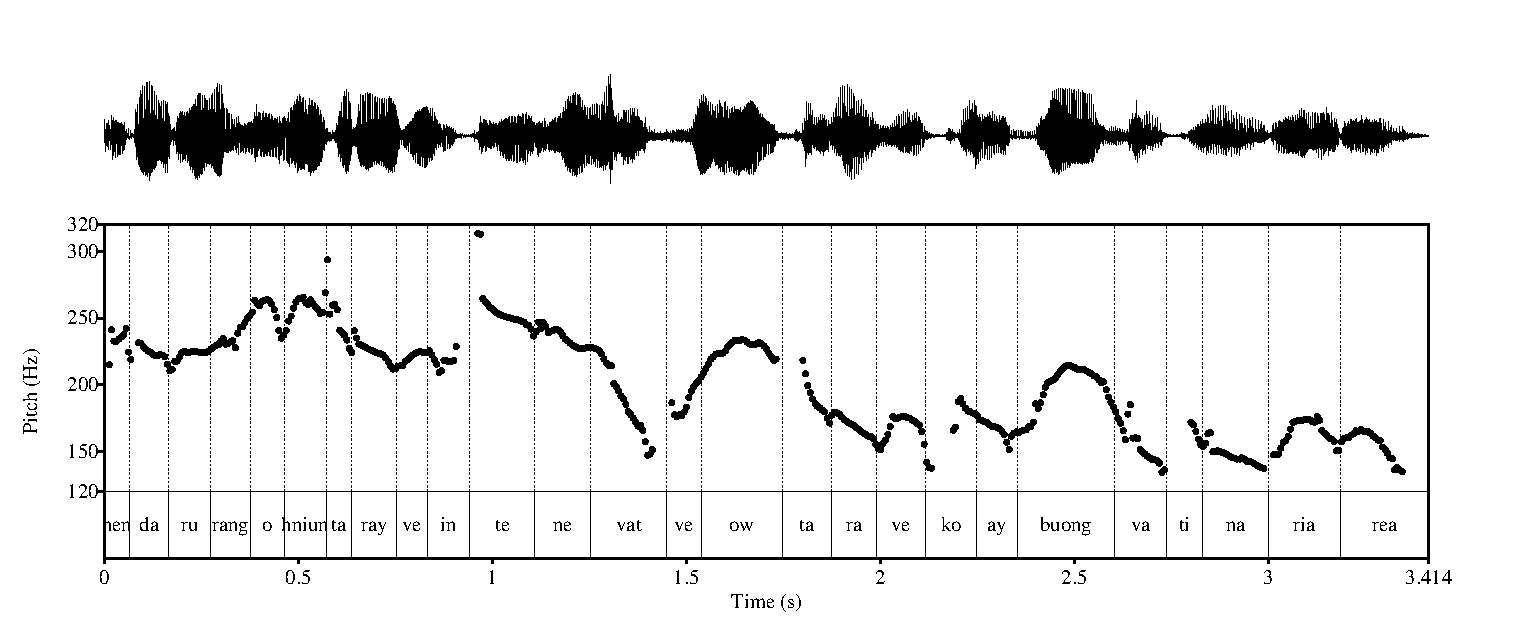
\includegraphics[width=\textwidth]{figures/pearOniLATCH.eps} 
\caption{F$_0$ contour of example (\ref{Wooi_Oni})}\label{fig:Wooi_Oni}
\end{figure}

\ea \label{Wooi_Oni}
\langinfo{Wooi}{Austronesian, SHWNG}{WBW\_pear\_Oni}
\ea
\glll henda rurang o: hniuntaray ve intene vat \\
he-ra rurang o: hniuntaray ve intene vati \\
3\textsc{pl}-go parallel \textsc{fill} person \textsc{rel} earlier \textsc{det}:\textsc{sg} \\
\glft `They walked alongside the man from earlier.' \\ 
\ex
\glll ve owta ra ve ko aybuong vat naria rea \\ 
ve owta ra ve ko aybuong vati naria rea \\
\textsc{rel} climb go \textsc{rel} take fruit \textsc{det}:\textsc{sg} again  \\
\glft `the one who climbed up who took the fruit again.'\\ 
\z
\z

Furthermore, the opposite assumption is not true either. There are in fact coherent intonation contours that exhibit internal pauses. Pauses are therefore not automatically a cue for a phrase boundary: When a speaker hesitates at a certain point the f$_0$ value at cut-off may be remembered and resumed at exactly the same level after the pause. This is to be understood as a continuation and not as a phrase boundary. Consider the following example from another Wooi pear story narration. In contrast to the case in (\ref{Wooi_Oni}) above, the speaker resumes the intonation contour at almost exactly the same pitch level as it was on \textit{na} right before the hesitation pause (if one were to cut out the pause, both ends of f$_0$ would fit together quite well).

\begin{figure}
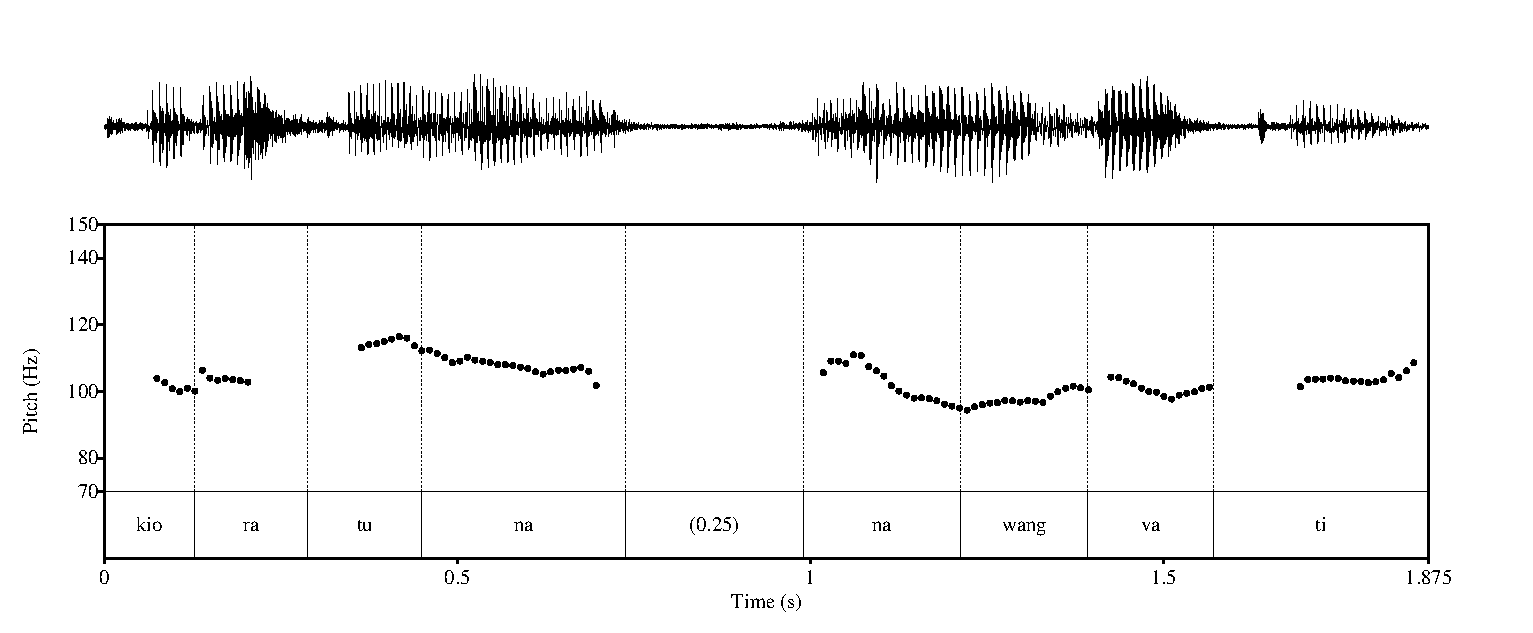
\includegraphics[width=\textwidth]{figures/pearJohnHESIT.eps} 
\caption{F$_0$ contour of example (\ref{Wooi_John})}\label{fig:Wooi_John}
\end{figure}

\ea \label{Wooi_John}
\langinfo{Wooi}{Austronesian, SHWNG}{WBW\_pear\_John}\\
\glll kio ra tu na (0.25) nawang vati \\
$<$i$>$ko ra tura na (0.25) nawang vati \\
$<$3\textsc{sg}$>$take go stand \textsc{loc} (0.25) basket \textsc{det}:\textsc{sg} \\
\glft `He took (them there and) left (them) in the basket.' \\ 
\z

So, to conclude at this point, the observation behind these arguments is that prosody seems to indirectly cue the existence of SVCs. There is certainly some sense in this argument if we look at 'minimal pairs' such as the one given by \citet{schapper2009bunaq} for Bunaq:

\ea \label{bunaq2}
\langinfo{Bunaq}{Papuan, TAP}{\citealt[442]{schapper2009bunaq}}\\
\gll Markus bola wa rebel \\
Markus ball discard descend \\
\glft `Markus threw the ball away downwards.’ or `Markus threw the ball away, (and he went) downwards.’\\ 
\z

Depending upon prosodic output, the example in (\ref{bunaq2}) may have two quite different readings. If uttered under a `single' intonation contour with a high boundary tone aligned to the first syllable of \textit{rebel}, the construction is interpreted such that it is the ball that descends. However, if there is a prosodic `break' between \textit{wa} and \textit{rebel}, and a final high tone is aligned to \textit{wa}, the interpretation is that it is Markus that descends after discarding the ball (thus making it two distinct event frames) \citep[442]{schapper2009bunaq}.

There is, however, a shortcoming with this argument. If a coherent f$_0$ always cues an SVC and an `incoherent' contour automatically precludes an SVC interpretation, then it would follow that the prosody - syntax mapping is exactly one to one. This would be a challenge for already established syntactic units such as the monoverbal clause. We know that clauses do not always neatly align with prosodic phrases (neither with \textsc{IP}s nor with intermediate phrases; see on this point e.g. \citealt{chafe1994discourse}, \citealt{himmelmann2006challenges}, \citealt{ladd2008intonational}, also \citealt{engelhardt2010}), and, indeed, I do not think that it is an exaggeration to claim that we do not know of \emph{any} syntactic unit with a constant prosodic output. Even if, ideally, speakers attempted to match syntactic clauses with coherent prosodic units, natural speech would always remain imperfect. As every field linguist is well aware, ``the physical manifestations of psychologically relevant units are always going to be messy and inconsistent" \citep[58]{chafe1994discourse}. Therefore we would expect that the prosodic chunking of SVCs is subject to variation just as it is found with other syntactic units. Seen this way, the explanatory power of the prosodic argument seems to be less strong and less reliable as is suggested by the standard reading in the literature. While there might be a partial correspondence between prosodic phrases and SVCs no exclusive argument can be based on prosodic behaviour. Yet, as this criterion is almost always used in order to determine SVCs, it has been adopted in the present study for practical considerations (see section §\ref{sec:defining} for discussion).

\subsubsection{Cognitive properties} \label{sec:cognitive}

The last parameter pertains to the cognitive background of SVC construals. It is claimed that SVCs express on the grammatical level what is on the cognitive level perceived as a single event. This claim is probably also the most controversial one and has been dismissed or called into question by many authors. What does event mean? One word of caution is in order here. There are at least two meanings of `event' in linguistics. What the typologists and descriptive linguists working on serialisation mean by `event' is quite different from what semanticists have in mind: the latter use is probably older, dating back in its modern sense at least to Zeno Vendler's verb class analysis \parencite{vendler1957verbs}. Here, event refers to a class of verbs (to the exclusion of stative and activity verbs) that can be deduced by testing their lexical aspect. Events in this sense are roughly equivalent to `dynamic verbs', or to `dynamic events' in Haspelmath's \citep{haspelmath2016serial} sense. 'Events' in the serialisation debate are not clearly defined but, very roughly, pertain to chunks of space and time in which something is happening (for instance, a basket of pears is stolen, or a pig is dying) and this something is perceived as having a starting point and an end point. So far so good. The trouble starts when it comes to the question of how these delimiters can be detected. Aikhenvald's definition patently demonstrates the challenge of this question:

\begin{quote}[S]emantically, serial verb constructions may encode one event, or several subevents closely linked together, or even several subevents in sequence which may be conceptualised as connected to each other. In the latter case, it may appear hard to draw a tight semantic distinction between a monoclausal serial verb construction and a sequence of clauses. \citep[12]{Aikhenvald2006}\end{quote} 

There are several problems with this definition, both terminological and theoretical. First, we encounter two different concepts: events and sub-events. What is the relationship between events and subevents? Does every event consist of subevents, and if so, of how many\footnote{Aikhenvald speaks of ``indissoluble" events which implies that there might also be events without a compositional structure \citep[12]{Aikhenvald2006}.}? What sounds like a part-whole relation is actually not defined by theory (see also \citealt[499]{bohnemeyer2007principles} on this point). If we by analogy compare events with syntactic units like a VP one could wonder whether events are also projected by subcomponents, that is, whether events are hierarchical in ways similar to constituent structure in syntax or to phonological structure. Yet there has been no real attempt in the serialisation debate to address such questions. 

A further terminological problem with Aikhenvald's definition arises with the phrases `subevents closely linked together' and `subevents [...] conceptualised as connected to each other'. What exactly is the difference between subevents being linked together and subevents being (conceptually) connected? As long as such notions cannot be made operational and useful to typological approaches, nothing is gained by including such claims into definitions of a phenomenon that is in and of itself only vaguely characterisable. Obviously, what authors have in mind when they speak of subevents is plainly the lexical condensation points of human event perception and segmentation, that is, verbs. My impression is that `different subevents connected together' is often interchangeable with `different verbs connected together'. \citet[15]{haspelmath2016serial} makes a similar point in remarking that

\begin{quote}[a]s far as I can tell, whenever a clear contrast between a single event and multiple events has been noted, it makes the same distinction as the grammatical criteria, in particular
monoclausality and biclausality.\end{quote}

He then concludes that the event parameter is not a necessary criterion for SVC determination. While that is certainly right at this point, I want to introduce very briefly two approaches that have tackled the event concept from different angles. The question that Bohnemeyer and colleagues \citep{bohnemeyer2007principles, bohnemeyer2011} posed was: How should linguistic event segmentation be measured?. Instead of matching event boundaries with syntactic or prosodic boundaries, they took the temporal frame of event expressions as their starting point and developed the 'macro-event property' (MEP). A MEP is defined as follows:

\begin{quote}A construction has the MEP if temporal operations such as time adverbials, temporal clauses, and tenses necessarily have scope over all subevents encoded by the construction. \citep[497]{bohnemeyer2007principles}\end{quote}

Whether or not a given construction has the MEP can be tested by applying a temporal operator. Thus, in the following example from \citet[503f.]{bohnemeyer2007principles}, (\ref{bohne1}) has the MEP, but (\ref{bohne2}) does not.

\ea
\ea
\label{bohne1} Floyd went from Rochester via Batavia to Buffalo.
\ex *Floyd went from Rochester at seven via Batavia at seven forty-five to Buffalo at eight thirty.
\ex \label{bohne2} Floyd left Rochester, passed through Batavia, and arrived in Buffalo.
\ex Floyd left Rochester at seven, passed through Batavia at seven fortyfive, and arrived in Buffalo at eight thirty.
\z
\z

While temporal modification of each constituent is fine with the multiclause example in (\ref{bohne2}), it does not work with the monoclausal event conceptualisation. Modifying each PP with a temporal operator sounds odd to English speakers, and signals according to Bohnemeyer et al. that the whole construction has the MEP.

Another approach to identifying event boundaries comes from neuropsychological research, methodologically established by \textcite{newtson1976perceptual}\footnote{Many thanks to Rebecca Defina for pointing that out to me.}. \textcite{zacks2007event}) and \textcite{zacks2010we} report findings from perceptual psychology and cognitive neuroscience showing that humans make use of automatic and incremental event segmentation in order to help predict what comes next and to cope with narrow information uptake \citep{zacks2010we}. In one experiment, participants watched films of everyday activites and had to press a button whenever they felt there was an event boundary. They did this twice. One time they were asked to segment the smallest meaningful event units, and another time they were asked to segment the largest units that were meaningful to them. The results were so consistent that it was argued that they show naturally occurring perceptual processing \citep[80]{zacks2007event}. In other experiments, participants viewed the video clips passively the first time before they were asked to do the segmentation. The segmentation data were then compared to brain activity data. Such data seem to suggest that event segmentation is something that we humans do all the while when we actively engage with the world. However, as \citet[81]{zacks2007event} noted 

\begin{quote}there is evidence
that observers can adapt their performance of the buttonpressing
segmentation task based on situational needs. For
example, observers adjust the temporal grain of their segmentation
based on explicit instructions, the sort of information they
are trying to learn from a stimulus, and how much they know
about the activity they are watching.\end{quote}

We have seen in the introductory chapter that the ``all-new approach" sets out from the assumption that SVCs are essentially different from clause linkage types, and might therefore reflect underlying differences in event perception and construal. A recent study by \citet{defina2012conceptual} looked into memory effects associated with the use of different grammatical constructions, raising the question whether the use of SVCs might bear on the ability of speakers to recognise and retrieve events. Speakers from English and Avatime (an African language with extensive use of serialisation) were asked to memorise short video clips of putting and taking events. Defina and Majid showed that false recognition of putting and taking events was more likely in Avatime when speakers produced SVCs in a \textit{post hoc} event description, whereas English speakers showed no difference in event recognition with regard to different grammatical constructions. Such findings may suggest that speakers of serialising languages can group event elements together, and store them as event units.

Summing up this section, although evidence from cognitive research amounts to the understanding that event segmentation is a naturally occurring human task, it is still controversial how this is actually reflected in linguistic chunking. Bohnemeyer and colleagues propose that event chunks are basically defined by their inherent temporal properties. Thus, temporal modification seems to be the most reliable test so far in order to detect the boundaries of `deeper' mental units that are different from better known linguistic units such as the clause.

\subsection{Coherence or Composition} \label{sec:coherence}

In the previous sections, I discussed cues to SVC detection that are regarded as standard arguments throughout most of the contemporary literature. In the following sections, I will introduce some further concepts that are not directly used as cues but form a more general backdrop of reasoning. The first idea to consider here is the concept of coherence. What makes a string of elements a coherent construction? All arguments introduced above as part of the `standard list of arguments' are actually based on a notion of coherence. The verbs form a coherent syntagma (the clause) on the basis of a coherent prosodic pattern, a coherent cognitive conceptualisation, as well as a coherent set of referents that is turned into `shared' grammatical arguments. All this reveals an important presupposition that is not always made explicit: that SVCs indeed constitute a unit (or construction) and do not consist of juxtaposed clauses (or VPs). This coherent unit has been addressed by features from different linguistic levels assuming that the boundaries of the phenomenon show through the different layers of the language system (for instance by prosodic chunking). This direction is in line with the ``all-new approach" that I outlined right at the beginning of the introductory chapter. The premise is that this unit is different from the traditionally recognised linguistic units (monoverbal clause, biclausal sentence). 

The presupposition of underlying coherence is, however, not prevalent in all approaches. Mostly in older contributions, we find proponents of the ``nothing-new approach" that assume that there is, though covert, an asymmetry in the verbs' ranking and that two VPs are linked together in ways similar to complementation or subordination strategies in other languages. A good example for this line of reasoning is Seuren's proposal of serialisation as an instance of pseudocomplementation. He defines pseudocomplementation as follows \citep[196]{seuren1991definition}: 

\begin{quote} A pseudocomplement is a suppositious sentential complement, foisted on a verb whose meaning requires no such complementation, and expressing concomitant circumstance, purpose, or result. Pseudocomplements are opposed to proper complements, which are semantically required by the governing verb.
\end{quote}

Thus, in essence, what Seuren has in mind is an adjunct VP\footnote{as opposed to cases of lexically governed pseudocomplementation such as in \textit{John went fishing} versus \textit{*John walked fishing} where the verb \textit{go} allows for a pseudocomplement whereas other English motion verbs do not (see \citealt[197]{seuren1991definition}).} tied to a matrix VP by specific grammatical rules: first, ``a controlled deletion (or non-expression) of the subject of the pseudocomplement (let's call it Secondary Subject Deletion or SSD)", and second, (optional) ``tense and/or agreement copying from the higher verb" in order to explain double-marked verb strings \citep[197]{seuren1991definition}.

The pseudocomplement approach and similar takes on verb chains aim at saving the generativist model of a single clausal head. \citet{baker1989object} also argued for an analysis that would leave the basic assumptions of the by-then version of government-and-binding intact. Baker proposed a system of double $\theta$-marking where both V$_1$ and V$_2$ $\theta$-mark the shared object argument of a given SVC in any SVO language. One of the outcomes of his proposal was an asymmetry in the status of V$_1$ and V$_2$ with the former verb being a structural sister to the object argument, and the latter being its structural daughter. \citet{Durie1997} has argued convincingly against such an analysis, pointing out that Baker's approach is not consistent with the data.

Whatever the theoretical backdrop of composite approaches is, they do raise the question about what it is that makes us so sure that underspecified verb sequences really form a coherent unit, or even more specific, a construction, as the standard term serial verb construction has it. Although it appears from the contemporary literature on serialisation that the coherence side has won the day, the issue of composition will resurface in later chapters of this book, and we will ultimately see in chapter \ref{ch:discussion} that both coherence and composition do seem to play a major role in the formation of MVCs in EI.

\subsection{Construction and productivity}\label{sec:construction}

In what sense, then, are SVCs constructions? In contemporary linguistic theories, there are at least two definitions of construction, a loose one and a strict one. While the loose one is used more or less as a desriptive cover term for a grammatical unit that consists of several items (lexemes and formatives), the strict one has a more narrow definition. For instance, \citet[4]{goldberg1995constructions} defines a construction as follows. 

\begin{quote}Constructions are taken to be the basic units of language. Phrasal patterns are considered constructions if something about their form or meaning is not strictly predictable from the properties of their component parts or from other constructions. That is, a construction is posited in the grammar if it can be shown that its meaning and/or its form is not compositionally derived from other constructions existing in the language.\end{quote}

If SVCs are viewed this way, we would assume that the meaning of the construct contains more than just the sum of the verb meanings. In other words, understanding `construction' in its strict sense entails the postulation of non-compositional meaning in SVCs. Reconsider the Bunaq example in (\ref{bunaq2}) from section §\ref{sec:prosodic} above. There is two verbs in sequence, indicating a downward movement of the ball away from the actor. To make it non-compositional in Goldberg's sense, the construction would need to convey a meaning that cannot be inferred from the meaning of the two verbs expressed in isolation. Indeed, as we have seen, prosody may coerce two quite different readings. The utterance could either be interpreted as a complex motion event where it is the ball that descends. This entails a change in the alignment of syntactic function and semantic role (the theme-object of V$_1$ becomes the actor/theme-subject of V$_2$). Or, if prosodically phrased in a different manner, one might read the sequence as consisting of two events, both performed by one and the same actor (throwing the ball, and then going). If the claim is that reading 1 is preferred under a coherent intonation pattern, then one could argue that the construction as such selects the change in alignment, and neither of the verbs would suggest so when viewed in isolation. Indeed, there is good reason to adopt such a constructionist perspective on multi-verb strings, and I will assume in later chapters (in particular in chapter \ref{ch:constructions}) that there are underlying constructional schemes at work.

Yet, as far as I can see, the whole discussion of SVCs actually makes very little reference to the concept `construction' (other than carrying it in its name), and does little to explain the consequences that the term might entail in a strict sense. An exception is \citet{haspelmath2016serial} who explicitly refers to constructions. He puts it as follows:

\begin{quote}To fall under my definition, a serial verb construction must be a productive schematic
CONSTRUCTION such that the meaning of a concrete construct can be determined on the basis of the meanings of its parts and the construction meaning. This means that non-compositional combinations of verbs do not fall under the definition. (\citealt[6]{haspelmath2016serial}; emphasis by the author) \end{quote}

Strictly speaking, ``concrete constructs" that consist not only of lexical meaning components but also of ``constructional meaning" are to be considered non-compositional according to standard definitions in literature on constructions (see for instance \citealt{goldberg1995constructions, goldberg2006constructions, croft2001radical}). Understood from a constructionist point of view, Haspelmath's definition that ``non-compositional combinations of verbs" are not considered would probably leave \emph{no} SVC at all in his basket. This is in all likelihood not what he has in mind. Non-compositional in Haspelmath's sense rather seems to be equivalent to non-productive. This is, however, not exactly the same. There are both productive and unproductive SVCs in many languages but both types are non-compositional rather than compositional. Take for instance the position-action construction from Wooi (see discussion in §\ref{sec:position-action}).

\ea \label{}
\langinfo{Wooi}{Austronesian, SHWNG}{frogstory\_Kosmus}\\
\glll hninyong katung mey teti tatuva wona pi \\
hninyong katung $<$i$>$mahoy $<$i$>$tati tatuva wona pi \\
 child little $<$\textsc{3}\textsc{sg}$>$sit $<$\textsc{3}\textsc{sg}$>$peek along dog \textsc{det}.\textsc{sg} \\
\glft 'the child sat staring at the dog.'\\ 
\z

We find two meaning components at work: first, there is the meaning of the two verbs \textit{mahoy} 'sit' and \textit{tati} 'peek' (ignoring the postverb \textit{tatuva} for the moment). Second, there is a meaning component that directly resides in the construction: neither the semantics of the sit verb nor of the peek verb tell us that both events go on simultaneously. For Wooi speakers the reading of this construction is always that of assuming a position and doing something at the same time. Such non-compositional meaning components are most probably inherent in most, if not all, SVCs. So, as a consequence I would rather assume (\textit{contra} Haspelmath) that canoncial SVCs are inherently non-compositional.

Productivity is a further parameter that is often invoked. As Haspelmath put it, `good' SVCs are considered productive and schematic (which makes them different from lexicalised constructions such as Zwicky's dismissive \textit{go jump in the lake}; \citealt[9]{zwicky1990we}). Productivity seems to presuppose a construction with slots into which verbs from certain semantically or functionally defined classes may enter. A construction then is productive if it would minimally allow new verbs into one of its slots. If one wanted to get rid of someone, \textit{go leap in the lake} or \textit{go jump in the bathtub} would most probably not have the same effect as \textit{go jump in the lake} precisely because there is no slot available that would allow new items. While the thought of productive SVCs seems appealing at first, we do know of many examples from the literature where authors discuss limits to productive patterns. An oft-repeated pair of examples, one licit and one illicit, is from \textcite{sebba1987syntax}:

\ea \label{}
\langinfo{Sranan}{Creole, Atlantic}{\citealt[60]{sebba1987syntax}}
\ea
\gll a teki a fisi seri \\
(s)he take the fish sell \\
\glft `(S)he sold the fish.' \\ 
\ex
\gll *a teki a fisi bay \\ 
(s)he take the fish buy \\
\glft intended: `(S)he bought the fish.'\\ 
\z
\z

While taking the fish to sell it is fine, taking the fish to buy it is rejected by speakers of Sranan. Durie has referred to such limitations as ``the unacceptability of non-events" \citep[327]{Durie1997}, proposing that the latter sequence is not a proper ``stereo-typical schema" for event-types in that particular language. I do not want to call this explanation into question. Yet it seems plain that `productive' SVCs are not quite that productive and that there is a number of language-internal or crosslinguistic restrictions at work. Even constructions that seem to be among the most productive ones, such as the highly frequent motion-to-action construction in EI languages with a motion verb followed by an action verb, are somehow restricted. Rarely have I seen any example of a motion-to-action construction in the EI data that would not feature an action verb in V$_2$ where the action is brought about willingly and the actor is in full control of the situation. There is nothing like 'he went fell into the lake' or 'he went noticed the child' which suggests that the construction as such has a meaning component \textsc{go somewhere + do something volitionally}. This precludes a large class of verbs that come with a non-volitional or non-control reading.

Productivity is thus a problematic concept: first, it does have clear limitations as a result of which fully productive SVCs probably do not exist (see also \citealt[40]{sebba1987syntax}). And second, no author has to my knowledge tried to make productivity operational by using some measure of quantification. Is a construction productive if it allows, say, twenty different verbs into one of its slots? Or is a construction productive if it allows all verbs of one semantic class (or field)? And if so, how can we delimit the semantic class? As long as these questions are not answered it does not make much sense to speak of productive SVCs unless we only want to emphasize that they are different from fixed lexicalised chunks. Productivity (as so many other linguistic parameters) is thus rather a matter of degree than a matter of either/or\footnote{Enfield made a related point regarding symmetrical and asymmetrical constructions, claiming that the choice between `restricted' and `unrestricted' verb slots (or rather verb classes, as some authors misleadingly claim) is rather a matter of personal intuition than of objective criteria. He writes: ``Though the distinction open versus closed is ostensibly discrete, there is much range in what is taken by different authors to fall into one or the other type, illustrated, for example, by the possibility of positing `closed classes’ with as many as 100 items (in Dumo; Ingram’s chapter, 202), or even 600 items (in Ewe; Ameka’s chapter, 125)" \citep[449]{enfield2009review}.}.

Some authors even seem to conflate productivity with frequency. For instance, \citet{bril2004complex} in her discussion of ``frequency and productivity" of Oceanic SVCs gives a table on p. 9 that has the title ``productivity of serial constructions". Yet the values she assigns to the different constructions/languages in the table cells clearly belong to the quite distinct category of frequency (``rare", ``infrequent"). The same conflation reappears in the prose: ``In the languages of New Caledonia, serial verbs also vary from productive [...] to infrequent..." \citep[10]{bril2004complex}. While there is certainly an overall tendency of highly productive constructions to occur in high frequencies, this is not a strict correlation or entailment but rather epiphenomenal. Constructions that are frequently used are salient construals and therefore arguably tend to be made productive by high patterns of usage. And conversely, highly productive constructions are prone to be used in new contexts, which makes them all the more frequent. Yet this is not always the case. To give a simple example, directional MVCs in Wooi only feature three directional verbs in V$_2$ and a couple of motion verbs in V$_1$. Yet despite this very restricted productivity, this construction belongs to the most frequent construction types in that language. Depending on the text genre taken, frequency of occurrence can be as high as every second to third IP. In much the same vein, formulaic lexicalised SVCs with fixed content may occur in high frequencies depending on the specific communicative function. Therefore, efforts should be taken to discriminate carefully between these two variables.

\subsection{Symmetrical vs asymmetrical SVCs}

From productive SVCs and open versus closed verb slots it is only a tiny step to symmetrical and asymmetrical SVCs. It is one of the most widely used concepts in the serial verb debate that SVCs may either be symmetrical or asymmetrical whereby symmetry pertains to the relationship between the status of the verbs. The idea of symmetricity in serialisation was primarily developed by Aikhenvald (\citealt{aikhenvald1999serial, Aikhenvald2006}, though \citealt{sebba1987syntax} already speaks of fixed verbs and free verbs), and has since been used by many authors of descriptive studies (for EI language descriptions, see for instance \citealt{kratochvil2007grammar}, and \citealt{bowden2001taba}).

In \citet[5]{bril2004complex} we find the following delimitation: \begin{quote}Symmetrical serial constructions consist of several co-ranking nuclei which belong to an open class, none of them determining either the semantic or the syntactic property of another verb of the sequence, and all under equal scope of a negation marker.\end{quote}

The key components in this definition are: co-ranking nuclei, open class, not property-determining, and equal scope of negation marker. Asymmetrical SVCs, on the other hand, are made up of the following properties: \begin{quote}Asymmetrical constructions [...] comprise hierarchized nuclei (i.e. a head and a modifier). The head belongs to an open class, while the modifier may come from a smaller, closed class with a variety of meanings and functions (such as verbs expressing direction, motion, posture, property, cause-effect, aspect, modality, etc.).\end{quote}

What we can gather from these definitions is that we are dealing here with antagonistic feature pairs: co-ranking contrasts with hierarchized and open class with closed class (and large with small, apparently). The two other properties of symmetrical SVCs are not named in the definition on asymmetrical SVCs, but it is probably implied that they have the opposite value there: nuclei do determine the semantic or the syntactic property of another verb in asymmetric SVCs, and may show varying scope of a negation marker. In a later paper, \citet{bril2007nexus} explicitly stated that co-ranking is meant to be equivalent to ``coordinate constructions" while hierarchised is used for ``subordinate constructions", but this does not seem to be very elucidative either\footnote{In fact, it is not clear whether coordinate and subordinate in Bril's sense pertains to coordination and subordination of clauses or to something else. If to the former, one would end up with the confusing notion of clause combinations taking place within single clauses.}.

The terms 'co-ranking' and 'hierarchised' seem more or less equivalent to '(grammatical) status' in other work. \citet[22]{Aikhenvald2006} gives the following definition of symmetrical serial verbs:

\begin{quote}Symmetrical serial constructions are not 'headed' in the way asymmetrical ones are: all their components have equal status in that none of them determines the semantic or syntactic poperties of the construction as a whole.\end{quote}

While this sounds quite similar to what Bril defined (see above), there is an interesting difference: being on the same rank in Bril's understanding means that none of the verbs exerts semantic or syntactic influence on the respective other verb. In Aikhenvald's definition, being on the same rank means that none of the verbs determines the semantic or syntactic properties of the construction. Asymmetrical SVCs, on the other hand, 

\begin{quote}denote a single event described by the verb from a non-restricted class. The verb from a closed class provides a modificational specification: it is often a motion or posture verb expressing direction, or imparting a tense-aspect meaning to the whole construction.\end{quote}

This is then illustrated by an example from Cantonese in which a \textsc{take} verb combines with a motion verb whereby the latter ``provides directional specification to the SVC" \citep[22]{Aikhenvald2006}.

\ea \label{}
\langinfo{Cantonese}{Sino-Tibetan}{\citealt[21]{Aikhenvald2006}}\\
\gll lei$^5$ lo$^2$ di$^1$ saam$^1$ lai$^4$ \\
you take \textsc{pl} clothing come \\
\glft `Bring some clothes.'\\ 
\z

What is problematic with the symmetrical-asymmetrical approach, however, is that authors seem to deviate from each other when assigning SVCs to either group. A puzzling example is provided by \citet{kratochvil2007grammar} who presents the following construction as an example of a symmetrical SVC:

\ea \label{}
\langinfo{Abui}{Papuan, TAP}{\citealt[351]{kratochvil2007grammar}}\\
\gll mi me feng \\
 take come injure \\
\glft 'Bring to slaughter.' \\ 
\z

The sequence is made up of three verbs, a \textsc{take} verb, a motion verb and an action verb: presumably, the actor obtains some object and moves to some place suited for the final action to be carried out. Or does he/she have something in his/her possession \textit{while} moving to the place of slaughter? The first part of the construction looks just like the Cantonese example from Aikhenvald above, and it just receives the same translation, rendered into English by a monoverbal structure `bring'. While Aikhenvald considers \textsc{take} plus motion to be an asymmetrical construction, Kratochvíl describes it as being symmetrical \citep[351]{kratochvil2007grammar}:

\begin{quote}These verbs are of equal grammatical status; they do not show any dependency with respect to each other. This means that none of the verbs [...] is semantically `dominant'.\end{quote}

Two conclusions could be drawn from this disparity. Either roughly homologous constructions belong to different symmetricity classes in different languages, that is, while \textsc{take} plus motion is asymmetrical in Cantonese, the Abui construction belongs to the class of symmetrical constructions. This would come as a surprise, however, given that the English translations in both cases seem identical. Alternatively, we might conclude that the symmetricity criterion is as of yet not defined well enough to allow for crosslinguistic application. 

\subsection{Nuclear vs core-layer SVCs}\label{sec:nuclear}

Work on verb serialisation has quite often made use of the `layered structure of the clause'-model from RRG \citep{olson1981barai, foley1984functional, van1997syntax}. The clausal architecture in RRG is different from other approaches to constituent structure in that the clause is not analysed as a projection from the finiteness features of the main verb. Instead, three layers are assumed to be active in clause structure, each one having its own constituents and its own operators: the nucleus is the innermost layer, and basically consists of the verb(s) and further formatives together constituting the predicate\footnote{Note that predicate in this sense does not include any of the verbs arguments. The nucleus in Foley and Van Valin's design may also comprise more than one predicate allowing for multipredicate clauses (a view that is in conflict with most definitions of serial verbs that assume one (complex) predicate within what is considered one clause; see \citealt[77]{foley1984functional}).}. The next layer is the core where the arguments of the verb(s) are placed (hence `core arguments'). Around the core, the outermost layer called periphery subsumes non-core arguments (adjuncts, oblique arguments) and secondary participants in the event \citep[77]{foley1984functional}. This layered structure of the clause is claimed to be universally present in languages, and in comparison to immediate constituent-approaches the theory also draws on evidence from non-configurational languages \citep[78]{foley1984functional}.

What makes the layered structure of the clause so appealing to authors working on serialisation is that it provides a straightforward explanation for different argument verb patterns in these languages. Any layer is able to combine with another building block of the same type, that is, allowing combinations of nuclei, cores or peripheries. \citet[188]{foley1984functional} refer to these combinations as junctures. They write:

\begin{quote}A nuclear juncture is a construction with a complex nucleus. It is a single unit, and all core and peripheral arguments are arguments of this complex nuclear element. In core-level junctures two cores, each with its own nucleus and core arguments, are joined together to form a larger complex core. The peripheral arguments must be shared by both cores, as they form a single complex unit within the peripheral layer. Peripheral junctures involve the joining of two clauses with independent peripheries.\end{quote}

In nuclear-layer juncture and in core-layer juncture, the periphery is shared by both juncts and so the whole construction still forms just one clause. As there is further variation with regard to the status of the arguments (in nuclear-layer juncture all core-arguments are arguments of the complex nucleus while in core-layer juncture, each verb (nucleus) governs its own core arguments) two different types of serialisation structures have been mapped on this model: in nuclear-layer serialisation, two verbs stand in direct sequence (contiguous) surrounded by the core arguments (which are arguments of the complex nucleus, as defined above). In contrast, core-layer serialisation has two verbs in non-adjacent position where the arguments of each verb may be placed between them (either the object of the first verb, or the subject of the second verb). The following table from \citet{bril2004complex} gives a structural overview of both types.

\begin{table}
\begin{tabular}{ll}
\lsptoprule 
Nuclear-layer serialization & Core-layer serialization \\
\midrule 
\pbox[c]{0.5\textwidth}{\textbf{sVV(o)} \\
 I run catch (him) } & 
 \pbox[c]{0.5\textwidth}{ a) same-subject: \\ \textbf{sVsV(o)} \\
 I run I catch (him) \\  \\
 b) switch-subject: \\ \textbf{sVo(s)V} \\ 
 (o = s) I strike him (he) dies }  \\
\midrule
one single set of arguments & verbs share at least one inner argument \\
\lspbottomrule
\end{tabular}
\caption[Nuclear and core-layer serialization]{Nuclear and core-layer serialization, taken from \citet[4]{bril2004complex}.}
\end{table}

Two points seem crucial here. First, the surface structure differs with regard to the feature `contiguity'. A second difference pertains to the relation between arguments and verbs: in nuclear-layer serialisation both arguments are selected by the nucleus complex (if transitive). In core-layer serialisation, each verb selects the same actor argument (same-subject type) or the U argument of the first verb is selected as A by the second verb (switch-subject type). Consider the following example from Olson's \citep{olson1981barai} foundational discussion of Barai (Papuan):

\ea 
\langinfo{Barai}{Papuan, TNG}{\citealt[190]{foley1984functional}}
\ea \label{barai1}
\gll fu fi fase isoe \\
\textsc{3}\textsc{sg} sit letter write \\
\glft `He sat down and wrote a letter.' \\ 
\ex \label{barai2}
\gll fu fase fi isoe \\ 
\textsc{3}\textsc{sg} letter sit write \\
\glft `He sat writing a letter.'\\ 
\z
\z

In (\ref{barai1}), the two verbs \textit{fi} 'sit' and \textit{isoe} 'write' combine in a core-layer serialisation, the U argument of the second verb separates both verbs. In (\ref{barai2}), the same verbs are placed adjacent to each other and the arguments precede the nucleus complex hence we deal with nuclear-layer serialisation. Both constructions differ nicely with regard to their semantics, further motivating the claimed constructional difference.

\subsection{Further variables}

The last sections have addressed variables with quite different status. While coherence and productivity are claimed to be a property of all SVCs by most authors, symmetricity and the varying juncture levels have been discussed as internal variables, corresponding to different subtypes of SVCs. As we have seen in the preceding section, nuclear- and core-layer serialisation draws on a number of variables at a finer grain: contiguity is needed in order to detect nuclear-layer serialisation (no argument may intervene between the verbs). Another variable that is at least indirectly tied to Foley \& Van Valin's dichotomy of junct relations in SVCs is wordhood. In languages where serialised structures consist of verb roots within one phonological word, the arguments are typically placed outside the word. What follows from this is that single-word SVCs are necessarily also nuclear-layer constructions. 

Wordhood is not an uncontroversial property. Some authors exclude serialisation on the root level because they assume that compounding is a different process and belongs to a different linguistic tier. For instance, \citet[27]{vanstaden2008serial} argue very carefully for a distinction between verbal compounding and what they call complex serialisation. Others like Aikhenvald treat wordhood as an internal variable, stating that ``components of a serial verb construction may or may not form independent grammatical or phonological words" \citep[3]{Aikhenvald2006}.

Another variable that I have mentioned already is variation in the marking of the verbs. While hardly any language seems to allow for free variation in verb inflection patterns\footnote{Tidore, a Papuan language of Halmahera, which is included in the EI dataset, appears to represent the odd one out. Subject indexing inflection can be added to verbs or left out in what seems to be free variation (see \citealt{vanstaden2000tidore}).}, many languages employ different strategies in different constructions. If one does not exclude cases with differential marking altogether (by arguing that differences in inflectional status entail hierarchical differences within the construction), at least two distinct values are possible here: constructions where all verbs are treated alike, and constructions where we find differences between the verbs. As we have seen in  Chapter \ref{ch:area}, many EI languages show irregular or unstable inflection patterns that are phonologically or lexically conditioned. Other languages do not even have verbal inflection systems. These are clear obstacles to applying this variable crosslinguistically.

Before closing this section, I would like to mention briefly another language compartment that is associated with the communication of event expressions. Recent work on gestures has suggested that co-speech gestures might be a useful tool for the detection of SVC boundaries. \citet{defina2016serial} showed for Avatime (Niger-Kongo) that while single gestures tend to overlap the whole SVC, clause-linking constructions are more likely to be associated with more than one gesture, overlapping single verb phrases rather than the entire construction. Such evidence will certainly make a valuable contribution to our understanding of serialisation, and might even help overcome the single event conundrum.

\section{Previous work on SVCs in Australasia} \label{previouswork}

The preceding sections have reviewed a set of criteria or variables that have been introduced in order to argue for external limits to and internal variation within verb serialisation. As I have tried to show, many of the variables are as of yet not operational in the sense that there are well-defined threshold values that researchers have agreed upon. Despite the ongoing debate on many of these variables, there has been considerable research into languages in EI as well as into neighbouring areas. 

In the following sections of this chapter, I will have a look at this research and approach the question how these variables have been put to use for language families in and around Eastern Indonesia. I will first discuss the results of Bril's research into Oceanic languages, then review van Staden \& Reesink's work on Eastern Indonesian languages, and finally introduce Pawley's analysis of Kalam, one of the most remarkable serial languages. All three approaches have in common that they propose new ways of ordering SVCs into classes. Bril has argued for a discrimination between co-ranked and hierarchized constructions, van Staden \& Reesink have advocated a hybrid classification into four types (independent, dependent, co-dependent and complex serialisation), and Pawley has differentiated between compact and narrative serialisation in Kalam. These sections therefore not only serve as a short introduction into studies from Australasia, but aim at discussing the potential applicability of the proposed types.

\subsection{Bril: Co-ranked vs hierarchized}

Research into serialisation in Oceanic languages has produced a good number of publications (for instance, \citealt{durie1988verb, bradshaw1993subject, crowley1987serial, crowley2002serial}). Bril contributed to this research with her papers on \textit{Complex nuclei in Oceanic languages: Contribution to an areal typology}  \citep{bril2004complex} and \textit{Nexus and Juncture Types of Complex Predicates in Oceanic Languages} \citep{bril2007nexus}. Drawing on a number of variables from other authors (like Foley and Van Valin's distinction into nuclear- and core-layer constructions), she developed a further subdivision into co-ranking versus hierarchized SVCs. 

Bril defines co-ranking constructions in Oceanic languages as follows:

\begin{quote}Co-ranking predicates belong to an open class; none of them determines the semantic or syntactic property of another predicate of the sequence. They generally refer to sequential actions done by the same agent as well as action-goal. \citep[269]{bril2007nexus} \end{quote}

This definition touches upon some of the notions from the preceding sections: Predicates (or verbs) belong to an open class, implying a symmetrical relationship in this sense (which is also expressed via the term `co-ranking'); and there is no mutual dependency between the predicated (verbs). These features are in contrast to the second category, hierarchized SVCs:

\begin{quote}Hierarchized predicates comprise a main verb (the head) and a modifying verb that do not obligatorily share the same subject [...]. The scope of the modifying predicate is either on the main verb or on one of the arguments of the main verb (in the
depictive type). \citep[270]{bril2007nexus}\end{quote}

These two types are not specified with regard to inflection patterns, adjacency configurations or operator scope. While the latter is assumed to be shared by all verbs, adjacency (or contiguity) of constituents is part of the juncture type distinction into nuclear-layer vs. core-layer on a higher level, that is, both nuclear-layer and core-layer constructions could be co-ranked or hierarchized.

Assuming that these two types are crosslinguistically extant constructions in the Oceanic languages, Bril admits that a discrimination between co-ranking and hierarchising is not always straightforward. If activity verbs are serialised, contextual factors are needed in order to disambiguate the intended reading. For instance, the combination of a motion verb and a verb of searching could in principle receive two different readings. Consider the following example from Pileni which may either translate as `paddle in (order to) search (at some place)' or `paddle searchingly' \citep[271]{bril2007nexus}:

\ea \label{}
\langinfo{Pileni}{Austronesian, Oceanic}{\citealt[271]{bril2007nexus}, quoted from \citealt[233]{naess2004serial}}\\
\gll Na no ua hehega na ko matu tuohine na \\
\textsc{3}\textsc{sg} \textsc{ta} paddle search \textsc{dem} \textsc{top} \textsc{1}\textsc{pl}.\textsc{ex}.\textsc{poss} sister \textsc{dem} \\
\glft `He has paddled here in search of our sister.’\\ 
\z

On the other hand, whenever a stative verb takes part in a SVC, it forms a hierarchized construction together with a main verb. This also follows from the assumption that the modifying verb has scope over the other verb or over one of its arguments. Stative verbs have a somewhat special status in the serialisation debate. While for instance \citet{haspelmath2016serial} opts to exclude stative verbs altogether, other authors tend to include them but often treat them as part of a special class (for example as minor verbs in asymmetrical serial constructions, or as ambient serialisation with concomitant predicate-argument configurations (see also the discussion in Chapter \ref{ch:gram})). 

In the Oceanic languages, there are three morphological operations that derive serialised stative verbs. These are: (i) transitive concord, (ii) causative or adverbial derivation, and (iii) reduplication. This makes the Oceanic languages different from most other serialising languages with underived insertion of stative verbs. In all three operations the stative verb takes a morphological marking that is not semantically tied to its lexical meaning but to the construction as such and functions as a constructional flag rather than a `real' semantic derivation of the stative verb. As Bril put it, ``[t]his derivation does not create a lexical class of adverbs, but marks the modifying/adverbial function of the stative V2" \citep[273]{bril2007nexus}. Here are some examples from different languages:

\ea \label{pileni}
\langinfo{Pileni}{Austronesian, Oceanic}{\citealt[272]{bril2007nexus}, quoted from \citealt[236]{naess2004serial}}\\
\gll Kolu-no maoli la khoulua kip-ina themu-ina \\
\textsc{2}\textsc{du}-\textsc{ta} true \textsc{dem} \textsc{2}\textsc{du} keep-\textsc{tr} quiet-\textsc{tr} \\
\glft `If you are telling the truth, keep it quiet.’\\ 
\z

\ea \label{hoava}
\langinfo{Hoava}{Austronesian, Oceanic}{\citealt[273]{bril2007nexus}, quoted from \citealt[162]{davis2003grammar}}\\
\gll Koni ome va-leani-a goe \\
\textsc{fut} see \textsc{caus}-good.\textsc{tr}-\textsc{3}\textsc{sg} \textsc{2}\textsc{sg} \\
\glft `You will see it well.’\\ 
\z

\ea \label{saliba}
\langinfo{Saliba}{Austronesian, Oceanic}{\citealt[275]{bril2007nexus}, quoted from \citealt[135]{margetts1999valence}}\\
\gll Ku-hedede-nogo-nogowai! \\
\textsc{2}\textsc{sg}-tell-\textsc{red}-slow \\
\glft `Speak slowly!’\\ 
\z

In the first example from Pileni in (\ref{pileni}), the second verb \textit{themu} receives the same transitive marking as the first verb \textit{kip}. It seems clear that the stative semantics of \textit{themu} is not modified into anything like `you quiet it' in a transitive sense. Rather, what happens is that the construction seems to impose on the stative verb the restriction to appear with the same transitivizer suffix as the first verb. Bril refers to this process as transitive concord and stresses that transitivised stative verbs only ever appear in SVCs but never occur on their own.

In the next example from Hoava, a similar effect is achieved by modifying the stative verb with what looks formally like a causative prefix in that language. Here as well, Bril emphasizes that the causative prefix does not target the meaning of the stative verb \textit{leani} `good', that is, the reading would not be `You see (you) cause it to be good' but rather `You see it well'.

The last example from Saliba illustrates the third operation. Here, the stative verb is reduplicated in V$_2$, a structure that looks much like adverb derivation in other languages. Bril again notes that ``[i]t is not a lexical but a derivational device marking the modifying function of the V2 and its syntactically dependent status" \citep[273]{bril2007nexus}. The difference between this and adverb deriving operations, such as the addition of \textit{-ly} in English, seems slight indeed, and rests upon the assumption that `slow' in Saliba is a verb and not an adjective.

Bril's dichotomy into co-ranked and hierarchized constructions is most clearly applicable in cases with stative verbs showing transitive concord. Concord of this kind may be marked by formatives derived from or related to causative affixes, transitivizers, or reduplication. While all these morphological devices are also in use in various languages of EI, I have not found any structural correlation of 'transitive concord'. Given that these clear-cut cases are seemingly absent, Bril's distinction into co-ranked and hierarchized constructions would produce a high number of ambiguous constructions in EI (in the same way as Bril discussed ambiguous combinations of activity verbs). Therefore, in order to capture Bril's intuition that there is a distinction between what may be called juxtaposition and modification further operational criteria would need to be found. In the next section, I turn to Miriam van Staden and Ger Reesink's approach to classifying SVCs. As we will see, their concept is quite different from Bril's and comes without explicitly dealing with modifying relations in Bril's sense.

\subsection[Van Staden/Reesink: Independent, dependent, ...]{Van Staden/Reesink: Independent, dependent, co-dependent, complex%
\subsectionmark{Van Staden/Reesink: Independent, dependent, ...}}
\subsectionmark{Van Staden/Reesink: Independent, dependent, ...}

In their study \textit{Serial verb constructions in a linguistic area}, \citet{vanstaden2008serial} investigated a sample of 12 serialising languages from Eastern Indonesia (six Austronesian languages and six Papuan languages) in order to explore potential genealogical and areal relationships. Their study covered much of the area that is also investigated in the present work, with the major exception of Sulawesi. Nine of the languages that van Staden and Reesink took as a sample are also part of my data corpus and reappear in this study. 

Adopting a rather inclusive definition of serial verb constructions, the authors counted all instances in which ``two or more verbs occur in a single clause and none of the verbs is apparently formally subordinated to the other" \citep[22]{vanstaden2008serial}. The potential ambiguity between serial verbs on the one hand and auxiliaries and prepositions on the other hand were ignored. However, cases of verbal compounding were excluded on the basis of prosodic evidence. 

The remaining cases are argued to fall into the following four classes: (i) independent serialisation, (ii) dependent serialisation, (iii) co-dependent serialisation, and (iv) complex serialisation.\footnote{The authors discuss another distinction into two broad types of SVCs, namely, component and narrative SVCs. The main defining feature of the former is Bohnemeyer et al.'s `macro-event property'. As this has been already discussed in the previous section, and because the exact discrimination between the two types is not entirely clear to me, I will not discuss this distinction here. Note that it does resemble Pawley's compact vs. narrative SVC approach (see next section).} While all four types are distinguished by their morphosyntactic structure, the classification is somewhat hybrid as the third type (co-dependent serialisation), as we will see, may either occur in an independent configuration or as an instance of dependent serialisation.

Independent serialisation describes the prototypical case where all verbs are equipped with the same inflectional morphology, and thus resemble an asyndetic coordinating structure. That independent serialisation is indeed not an instance of asyndetic coordination is established by language-specific properties. The authors suggest:

\begin{quote}For one language, this may be the scope of negation or placement of negation particles, for another it may be the radical change in meaning when a conjunction is inserted, or a characteristic prosodic contour. \citep[23]{vanstaden2008serial}\end{quote}

Such an approach is in stark contrast to the typological claim made for instance by \citet{haspelmath2016serial} that SVC identification must be based upon criteria that can be put to the test by applying the same operation across all languages. For van Staden and Reesink, it seems to suffice to draw on, say, prosodic evidence in one language, and on operator scope in another. The advantage of being liberal in the general definition of what to count as a serial verb is thus minimized by allowing for all kinds of further properties on the individual level of the language in question. A further problem arises with isolating languages where no choice of constructional inflection patterns can be made \citep[23]{vanstaden2008serial}.

Dependent serialisation covers those constructions in which one of the verbs carries all verbal inflection, and the other appears in its bare or stripped-down form. As the bare verb does not have finiteness features, this type thus formally resembles subordinate structures or auxiliary constructions \citep[24]{vanstaden2008serial}. Subordinate or auxiliary interpretations are ruled out in cases where there is no clear evidence in favour of such an analysis. The following example from Hatam has two dependent serialisation constructions, both of which show asymmetrical inflection patterns across the verbs (for instance, \textit{kwei} takes inflection but not \textit{buwak}).

\ea \label{}
\langinfo{Hatam}{Papuan, Hatam-Mansim}{\citealt[24]{vanstaden2008serial}}\\
\gll di-kwei buwak di-sutbatnya i-bou poi bu ba i-bit da ba n-ug ngat ei bigbehei \\
\textsc{1}\textsc{sg}-come gather \textsc{1}\textsc{sg}-friends \textsc{3}\textsc{pl}-head few again and \textsc{3}\textsc{pl}-follow \textsc{1}\textsc{sg} and \textsc{1}\textsc{pl}.\textsc{ex}-go see \textsc{loc} forest \\
\glft `I came (and) got a few of my friends together again and they'd follow me and we'd go look in the forest (for game).'\\ 
\z

Co-dependent serialisation, as I have already indicated, crosscuts the previous distinction into fully-inflected vs. partially inflected SVCs. Here, it is not the inflection pattern but the argument configuration that is the defining criterion. Co-dependent serialising constructions invariably share one argument and each verb makes use of this argument in a different syntactic function: this pivot argument is the object of V$_1$ and the subject of V$_2$ (corresponding to the switch-function or switch-subject type in \citealt{Aikhenvald2006} and elsewhere). While this type seems most often restricted to causative or cause-result semantics (the object denoting the patient or theme which then is reanalysed as the subject of an unaccusative verb to specify the result of the action, the \textit{x hit y (y) die} type), van Staden and Reesink also note other uses of co-dependent serialisation patterns. For example, they cite cases from Moi where the construction seems to be in use in directional and in instrument constructions.\footnote{The examples given for Moi seem strikingly ambiguous between a switch-subject reading and an ambient reading where the subject of the second verb is not the object of the first one but in fact the whole predicate. Looking at the example of instrument use,

\ea \label{}
\langinfo{Moi}{Papuan, WBH}{\citealt[26]{vanstaden2008serial}, quoted from \citealt[51]{menick1996verb}}\\
\gll w-aala ton p-ai sin-keelik \\
\textsc{3}\textsc{sg}.\textsc{m}-cut first \textsc{3}\textsc{sg}.\textsc{nhum}-'with' knife-machete \\
\glft `First, he cut it with a machete.'\\ 
\z

one could wonder if at all there is a reading available in which the subject indexer on the second verb takes up the (covert) object. This would have to yield something like `he cut it$_i$, (it$_i$) was with a machete', thus resembling a comitative argument status of \textit{sin-keelik} rather than an instrument one.}

Complex serialisation is the last SVC class in van Staden and Reesink's framework and refers to cases where two or more verbs share one set of affixes (the prefix attaching to the first verb and the suffix to the last one). In this sense, the definition corresponds to the surface structure of Foley and Van Valin's \citep{foley1984functional} nuclear-layer serialisation \citep[26]{vanstaden2008serial}. Example (\ref{ambon}) from Ambon Malay illustrates the difference between a co-dependent construction and a complex SVC.

\ea \label{ambon}
\langinfo{Ambon Malay}{Creole}{\citealt[41]{vanstaden2008serial}, quoted from \citealt[56]{tjia1997verb}}\\
\ea \label{ambon1}
\gll be pukol anjing mati \\
I hit dog die \\
\glft `I killed dog (by hitting).' \\ 
\ex \label{ambon2}
\gll be pukol mati anjing \\ 
I hit die dog \\
\glft `I killed dog (by hitting).'\\ 
\z
\z

Both constructions are reported to differ in the focus that is on the constituents. In (\ref{ambon1}) the emphasis is on the result (\textit{anjing mati}), while in (\ref{ambon2}), the focus shifts to the ``manner in which the state change is brought about" \citep[41]{vanstaden2008serial}, that is, \textit{pukol mati}. While from a structural viewpoint two different constructions may be identified, the focus difference may as well reflect a more general trait of Ambon Malay, pertaining to the focus potential of different post-verbal positions (for instance, the first case could be analysed as having a filled clause-final focus slot, highlighting the resultant state, while the second configuration would feature an `incorporated' second verb as part of the main predicate). The question remains whether this information structural difference would only occur in SVCs or reappear in other construction types as well.

Now, if we look at these four types, it becomes obvious that we are not just dealing with one variable but with at least three: (i) inflectability of the verbs distinguishes independent from dependent serialisation; (ii) the functional switch in the pivotal argument is associated with co-dependent serialisation but may in fact occur with all three types (for instance as complex serialisation in (\ref{ambon2})); (iii) adjacency of verbs is a prerequisite for the affix sharing complex serialisation. Adjacency is not relevant, however, to any of the other three types, nor is inflectability relevant to co-dependent and complex serialisation though in the latter case the inflection pattern does play a role. Thus, in independent serialisation only inflectability has to have a specific value (all verbs inflected), while the other two variables may occur either way. The same is true for dependent serialisation. Co-dependent serialisation is orthogonal to the other three types as the switch-function value is optional for all types but for co-dependent serialisation. Complex serialisation can also be viewed as orthogonal if (verbal) adjacency is the defining variable. 

Concluding, it would seem more beneficial to deconstruct these four types into their key defining variables and annotate each case of SVC for all variables instead of dealing with the wealth of SVCs by means of orthogonal non-atomic feature configurations. 

\subsection{Pawley: Compact vs narrative}

The last approach to SVC classification to be discussed in this context is Pawley's and Lane's work on the Papuan language Kalam spoken in the Western Highlands Province of Papua New Guinea \citep{Pawley1987, pawley1991saying, pawley2008serial, pawley2011event, lane2008kalam}. Kalam is a language with many peculiar features, some of which have profoundly stimulated the debate on verb serialisation. Perhaps the most striking feature of Kalam is the organisation of the verbal lexicon. Quite unlike most languages of the world, Kalam has a rather small and closed class of verb stems comprising only about 130 members \citep[7]{lane2008kalam}. At the same time, a small portion of these verbs appear to have very broad and generic meanings, and these `generic' verbs contribute the bulk of verb tokens found in natural data (fifteen of these verbs account for 89\% of all verb tokens, and 35 of these generic verbs make up 98.6\%; \citealt[7]{lane2008kalam}). This scarcity of verb stems is obviously associated with a high frequency of varying types of serialisation patterns in Kalam. While most SVCs contain two or three verbs, the practical limit to verb concatenations seems to be at nine to ten verbs \citep[172]{pawley2008serial}. The wealth and complexity of serial verbs in Kalam thus by far exceeds most other serialising languages, as the following example illustrates.

\ea \label{kalam1}
\langinfo{Kalam}{Papuan, TNG}{\citealt[173]{pawley2008serial}}\\
\gll mj bep tk d ap nb okyang jok-l \\
leaf plant pick get come place below throw-\textsc{ss}.\textsc{prior} \\
\glft `Having picked, brought back, and tipped \textit{bep} leaves down (in an oven pit)...'\\ 
\z

Some further features of the Kalam verb systems are markedly different from most verb systems in Eastern Indonesia. First, apart from the small size of the vebal lexicon, Kalam makes use of clause-chaining (marking subject (dis)continuity by subject reference marking) with medial verbs heading all non-paragraph final (coordinate-dependent) clauses (for instance \textit{jok-l} in example (\ref{kalam1}). Thus, there are at least two multi-verb operations in Kalam, operating on different levels, that is, serisalisation and clause-chaining. Second, the inflected verb in both serialised verb sequences and clause-chaining constructions always comes last. Third, there is a class of uninflectible `verbal adjuncts'. These adjuncts may form a complex predicate with a full verb and behave like an adverb, yet their meaning is often similar to that of a full-flegded verb, and sometimes the adjunct may alter the argument configuration of the complex predicate (as opposed to adverbs; \citealt[177]{pawley2008serial}).

By classifying Kalam verb combinations into types, Pawley found that many verbs occur together in certain grammatically and semantically definable ways. These combinations usually comprise only two or three verbs and form a `compact' construction. 

\begin{quote}A compact SVC expresses a sequence of conceptual events that are tightly integrated, grammatically and semantically. Compact SVCs are strictly V-serialising, i.e. no other morphemic material can occur between the verb roots. The verbs in the SVC share a single argument structure and the scope of negation and modifiers is always over the whole SVC. Some, perhaps most compact SVCs cannot be readily paraphrased by a multi-clause construction. Many, though by no means all are translatable by a simple or phrasal verb in English. \citep[172f.]{pawley2008serial}\end{quote}

This definition bears resemblance to Van Staden \& Reesink's complex serialisation: the verbs are placed adjacent to each other, projecting a single argument structure. Though Kalam has its finite verb at the end of verb sequences, compact SVCs do not necessarily possess a `reversed' dependent pattern sensu Van Staden \& Reesink. This is because several compact SVCs can be combined to form what Pawley calls a narrative SVC, a larger serialised unit composed out of `nuclear' compact SVCs. In these larger concatenations only the final compact SVC bears inflection.

\begin{quote}Narrative SVCs provide a means for packing episodic reports into a single clause structure without omitting mention of any of the component events that Kalam discourse structure rules require of minimal well-formed event reports. Narrative SVCs can readily be paraphrased by multi-clause or multi-sentence constructions, where each clause specifies a distinct stage in the narrative action. Some narrative SVCs superficially resemble compact SVCs in that all the verb roots occur contiguously, without any intervening material. However, in syntactic terms narrative SVCs can be classed as VP-serialising. A clause of this class can be divided into two or more phrases each of which has a limited degree of grammatical independence. \citep[174]{pawley2008serial}\end{quote}

Compact and narrative SVCs are thus not on a par but constitute serialisation techniques on different syntactic levels. This approach enables a hierarchical analysis of SVC levels. Pawley gives the following example:

\ea \label{}
\langinfo{Kalam}{Papuan, TNG}{\citealt[171]{pawley2008serial}}\\
\ea
\gll basd skop am kmn pak d ap ad ñb-algb-al \\
g'father distant go animal kill get come cook eat-\textsc{pst}.\textsc{hab}.\textsc{3}\textsc{pl} \\
\glft `Our distant ancestors ... used to go, kill, bring back, cook and eat game mammals, ...'\\ 
\ex
$[[$go$]_{\textsc{vp}}$ $[[$game.mammal kill$]_{\textsc{vp}}$ $[$get come$]_{\textsc{vp}}$ $[$cook eat$]_{\textsc{vp}}$ $]_{\textsc{vp}}$ $]_{\textsc{vp}}$\\
\z
\z

The construction consists of two levels: a matrix narrative construction with two slots, a motion slot and another slot for the action. This action can be episodic in the sense that more than one event pattern is given in sequence. In this example, the second slot is filled by three `coordinate' compact SVCs: killing game mammals, bringing the game back home, and processing and eating it at home. Note that the three compact SVCs each have a different spatiotemporal frame: the killing is done in the woods, the bringing back connects the woods with the hunters' homes in the village, and the cooking and eating takes place in the village. Though Kalam is probably quite unique in adjoining so many compact SVCs, the multi-verb components (transport motion, cooking and eating, and, on the matrix level, motion-to-action) are all well-known also from the EI area, and the EI data set provides many examples of similar combinations (see Chapter \ref{ch:constructions}). Thus it seems likely that the building blocks that Pawley identifies for Kalam are at least in parts also existant in languages of EI. This in turn suggests that the process of forming these types, mediated by culture-specific experiencing of the surrounding world and shaped by frequency-based conventionalization (and perhaps, to a certain extent, lexicalization), is part of a more general pattern of event conceptualization, in the area of Eastern Indonesia and perhaps well beyond.

\section{Multi-verb constructions} \label{section:multi-verbconstructions}

The previous sections have dealt with serialisation as a theoretical concept, and the various ways authors have approached and defined the phenomenon. In §\ref{section:properties}, I focused on a set of components that are central to the most widely discussed definitions of serial verbs. As I have suggested, there are two types of parameters: independent parameters that can be assessed directly by applying some testing procedure, and dependent parameters that require the definition of yet another concept. Monoclausality is a good case in point. In languages like Kalam with specific clause-final verb morphology, clausehood may be accurately determined, but in many languages of EI, verbal inflection is absent or conditioned by phonological or lexical factors. In such languages, clausehood seems to be a concept that resists an easy definition. In §\ref{previouswork}, I reviewed three approaches to serialisation in the Australasian region. While all three approaches came up with new ways of classifying SVCs, their classificatory systems either rely on specific areal or language-specific features (Bril's co-ranked vs. hierarchized approach for instance worked best with transitive concord in SVCs with stative verbs), or on hybrid systems (as with van Staden and Reesink's four-way distinction).

The preceding discussion has shown that authors still struggle with finding the right set of delimiting criteria. What seems to work best for one language, turns out to be not applicable or even unwanted in another. It appears that the quest for watertight cross-linguistic definitions has led authors to include more and more pieces of evidence from different linguistic subsystems (think of prosody, or cognitive event construals). This profusion of criteria is only in rare cases fully applicable to a given language, and it is now more and more apparent that serialisation as a theoretical concept is far too laden with features that are hard to put to the test, while at the same time the phenomenon, as a whole, continues to have fuzzy boundaries. 

There are at least two reactions to this situation in contemporary literature on serialisation. The first reaction is to try and narrow down the inventory of defining features, sorting out those ones that are not operational (impractical in Haspelmath's terms) and thus hamper progress in cross-linguistic comparison. I have already reviewed Haspelmath's take on serialisation who claims to provide a definition that is ``considerably narrower than definitions used by most other authors" \citep[6]{haspelmath2016serial}. 

The other reaction is to avoid the concept altogether, and instead come up with a more neutral term. The alternative that has come to be used most widely in recent years, and that I will adopt in the following chapters, is `multi-verb constructions' (abbreviated MVC). For instance, Enfield in his discussion of verbs and multi-verb constructions in Lao explicitly refrains from using the term `serial verb construction' because it ``has been used in a range of ways in the literature [...], and may be too suggestive of certain specific types of construction which form only a subset of the broader set of expressions described in this chapter" \citep[104, footnote 17]{enfield2008verbs}. This is a motivation that is prominent in most authors preferring the use of the term multi-verb construction. The advantages include, first, avoiding the `inherited' bulk of literature on serial verbs and the many definitions, and second, taking into account a broader picture with constructions that would normally be neglected or disregarded as proper instances of serialisation. \citet[312]{nordhoff2012} is another proponent of this strategy:

\begin{quote}
[W]e find that many languages [of South Asia] also make use of constructions involving more than one verb, but they do not always fit within the definitions provided by either the Creolist or the general typological literature. This has to do with various markers of subordination like infinitives or participles [...]. To avoid possible confusion, I will use 'multi-verb construction' (MVC) as a general pretheoretical cover term for any construction with more than one verb [...].
\end{quote}

\citet{senft2008event} in his contribution on serial verbs in Kilivila also makes use of the term `multi-verb construction' as a hyperonymic concept, subsuming both serial verb constructions and what he calls contiguous serial verb constructions. He goes on to define MVCs in Kilivila as follows \citep[10]{senft2008event}: 

\begin{quote}Verbs constituting MVCs have shared polarity, but they need not have shared tense, aspect and modality, and they need not all refer to the same subject, either. MVCs are produced under a single intonation contour without internal pauses. MVCs are used not only to describe what is conceptualised as a single event but also what is conceptualised as a complex event or as an episode which may consist of both macro and subevents.\end{quote}

What is interesting here is that Senft (as well as other authors) does not dispense with difficult concepts like `single intonation contour' or eventhood altogether, but associates them with the hyperonymic term MVC while keeping the independent features argument sharing and same operator value for serialisation in the strict sense. This is a split of one concept into two concepts rather than a real gain for a multi-verb analysis as for both SVCs and `contiguous SVCs', evidence for coherent prosody and/or event boundaries would still need to be found.

Summarising so far, it becomes obvious that, as the discussion on SVCs produces more and more theoretical restrictions to the concept, writers have started to look for alternative concepts that are less restricted and applicable to a range of similar construction types that lack certain properties of canonical SVCs. One of the most frequent mismatches with `traditional' definitions involves operator values that are not necessarily shared across the whole construction. But, as Senft's definition bears witness, there are also other parameters that sometimes hardly fit with one's own data. The single event criterion is such a notorious obstacle, but this, as we have seen, is also called into question by authors that stick to the concept of serial verbs (like recently, \citealt{haspelmath2016serial}). 

\subsection{Literature and previous definitions} \label{sec:literature-mvcs}

Multi-verb construction is a new and largely undeveloped concept. Using the term, therefore, is both an advantage and a drawback. As the last section showed, researchers are in need of matching their data with existing concepts, and data on serial verbs often deviate from the standard definitions at some point. Therefore, starting from scratch may allow the inclusion of further data points that are intuitively felt to be related to canonical serial verbs, but show aberrant features. On the other hand, in order to make a new concept theoretically useful, clear limits have to be set, and ideally an explanation would have to be provided as to why the limits are where they are. 

In this section, I will look at the (so far) rare cases in which multi-verb constructions have been defined. As the quotations from the last section illustrate, some authors are just happy to have an `unspoilt' concept without rigid restrictions. Using the term that way is pretheoretical and descriptive, but of little help when it comes to discussing the relationship between it and already established concepts such as serialisation or complex predicates. Table \ref{table:multi-verb} below gives a list of features from three authors that have dealt with multi-verb constructions in a more explicit way.

\begin{table}
\begin{tabularx}{\textwidth}{l QQQ}
\lsptoprule 
Parameter & \citealt{ameka2005multiverb, ameka2006ewe} & \citealt{enfield2008verbs} & \citealt{Aikhenvald2011} \\
\midrule Clausehood & variable & variable & monoclausal \\
Predicatehood & -- & -- & single \\
Prosodic marking & -- & prosodically integrated unit & -- \\
Syntactic dependency & unmarked & -- & optional linker \\
Argument sharing & typical & -- & yes \\
Verb status & independent & -- & -- \\
\lspbottomrule
\end{tabularx}
\caption[Parameters used to define multi-verb constructions]{A comparison of parameters used to define multi-verb constructions in the literature.}
\label{table:multi-verb}
\end{table}

The first researcher who explicitly uses the term is, to my knowledge, Felix Ameka in his analysis of West African multi-verb constructions \citep{ameka2005multiverb, ameka2006ewe}. Taking one step back, Ameka includes under his definition of MVCs three subtypes: multi-clausal consecutive constructions with (optional) overt linkers between the clauses, overlapping constructions that are also biclausal but lack an overt linker, and monoclausal serial verb constructions. Both consecutive and overlapping constructions may have their constituents negated independently. The same goes for tense and aspect marking in consecutive constructions, but not so in overlapping constructions which need to share the same TAM values. It appears that consecutive constructions cover much of what is otherwise referred to as juxtaposed clauses or asyndetic clause-linkage, while overlapping constructions exhibit certain argument `sharing' configurations like object-to-subject or predicate-to-subject relations reminiscent of instances of non-canonical serialisation (like, for instance, Crowley's ambient serialisation). The term overlapping is apparently chosen because there is some conceptual connection between the clauses and their arguments. However, while van Staden and Reesink's term `co-dependent' comes to mind with examples such as (\ref{ewe2a}) below, Ameka differentiates between those cases and full-fledged switch-function SVCs as in (\ref{ewe2b}), as only the former type requires both subjects on the verbs to be expressed. Compare the following three examples that each denote two stages, the second of which could be interpreted as resulting from the first one. 

\ea \label{ewe1} 
\langinfo{Ewe}{Niger-Congo}{\citealt[18]{ameka2005multiverb}}\\
\gll tu-i né me-mé o \\
\textsc{2}\textsc{sg}-grind-\textsc{3}\textsc{sg} \textsc{consec} \textsc{3}\textsc{sg}:\textsc{neg}-fine \textsc{neg} \\
\glft `Grind it and let it be not too fine.'\\ 
\z

\ea 
\langinfo{Ewe}{Niger-Congo}{\citealt[27]{ameka2005multiverb}}\\
\ea \label{ewe2a}
\gll Kofi fo-e wò-dze anyí \\
Kofi strike-\textsc{3}\textsc{sg} \textsc{3}\textsc{sg}-contact ground \\
\glft `Kofi struck him/her (s)he fall down.' \\ 
\ex \label{ewe2b}
\gll Kofi fo-e fú anyí \\ 
Kofi strike-\textsc{3}\textsc{sg} hit ground \\
\glft `Kofi struck him/her down.'\\ 
\z
\z

Example (\ref{ewe1}) shows a consecutive construction. There is a linker \textit{né} present, and only the second clause is negated. In (\ref{ewe2a}), we get an overlapping construction for the reasons mentioned above. Adding a linker would not be possible here. And (\ref{ewe2b}) illustrates a serial verb construction proper as the second verb \textit{fú} fails to receive a subject indexer of its own. Clearly, all three of these instances could with some justification be analysed as some kind of multi-verb structure. The consecutive case does provide a formal connector between the clauses, yet it still lacks the difference in finiteness typical of subordinated clauses, and the use of the connector is optional, making it at best an asyndetic coordination (albeit with differing semantics, as the consecutive semantics are stricter and exclude, say, a simultaneous interpretation of some \textsc{clause and clause} structure.). 

Working on languages of Mainland South-East Asia with very little morphology, Enfield also makes use of the term multi-verb construction. In Lao, formally unmarked sequences of verbs are a common grammatical means. Yet \citet{enfield2008verbs} shows that most of these sequences can be dissected into (most often) binary pairs of (two) verbs that work conceptually as a unit. Take sentence (\ref{lao1}) below featuring six verbs in a row, all of them being prosodically integrated.

\ea \label{lao1}
\langinfo{Lao}{Tai-Kadai}{\citealt[83]{enfield2008verbs}}\\
\gll caw$^4$ lòòng$^2$ mèè$^4$ qaw$^3$ paj$^3$ hêt$^1$ kin$^3$ beng$^1$ \\
\textsc{2}\textsc{sg} try.out \textsc{ptl} take go make eat look \\
\glft `You go ahead and take (them) and try cooking (them)!'\\ 
\z

By applying different tests, the verb string may be resolved into two main relationships. \textit{lòòng$^2$}, a left-headed complement-taking adverbial, is in direct relationship with final \textit{beng$^1$} both of which form a bracket around a complex verb phrase denoting a process of object manipulation \citep[83]{enfield2008verbs}. Within this complex verb phrase, taking and going are closely related to each other (embedded directional into the taking event), as are making and eating (purposive relation). This example already sheds light on the way Enfield deals with such multi-verb structures. The one defining property of a verb complex to fall within the category of MVCs is full prosodic integration \citep[104]{enfield2008verbs}. Other properties, such as the range of grammatical features of canonical main verbs in MVCs, clause seperability, yes-answers, ellipsibility of object complements, insertability of left aspect-modality marking and insertability of a focus particle are cogently discussed as variation within the MVC category rather than delimiting features because MVCs in Lao show different reactions to these tests. Therefore, Enfield neither includes restrictions on the clausal status of such constructions, nor on other typical features such as predicatehood or argument sharing. To illustrate the range of variation, take a feature like ellipsis of verbs in a yes-answer. One strategy of affirmatively answering a Lao question is to repeat some portion of the question \citep[106]{enfield2008verbs}. Enfield shows that there  are roughly three types of answering behaviour depending on the MVC: repetition of V$_1$ (thereby eliding V$_2$) is preferred in cognitive complements (`see', `forget', `hear') and phase complements (`begin', `cease'). Other complement-taking verbs such as `want' permit both repetition of  V$_1$ and V$_2$ or repetition of `want' alone, as illustrated in example (\ref{lao2}). 

\ea \label{lao2}
\langinfo{Lao}{Tai-Kadai}{\citealt[107]{enfield2008verbs}}
\ea \label{lao2a}
\gll caw$^4$ jaak$^5$ paj$^3$ bòò$^3$ \\
\textsc{2}\textsc{sg} want go \textsc{ptl}.\textsc{q} \\
\glft `Do you want to go?' \\ 
\ex \label{lao2b}
\gll jaak$^5$ paj$^3$ \\
want go \\
\glft `(Yes, I) want to go.' \\
\ex \label{lao2c}
\gll jaak$^5$ \\
want \\
\glft `(Yes, I) want (to go).' \\ 
\ex \label{lao2d}
\gll paj$^3$ \\ 
go \\
\glft `(Yes, I want to) go.' (or - `(Yes, I'll) go.')\\ 
\z
\z

The typical answer to question (\ref{lao2a}) is to repeat both verbs, as in (\ref{lao2b}). However, shortened (\ref{lao2c}) is also acceptable, as is theoretically (\ref{lao2d}) (which, however, is ``arguably not a straight answer" \citep[107]{enfield2008verbs} to (\ref{lao2a})). Still other constructions prefer  repetition of only the second verb, such as combinations of motion-to-action sequences where only the action part is repeated. Thus, with this variation in mind, no savvy \textit{ad hoc} exclusion of one type in favour of another seems possible.

Aikhenvald follows a third strategy. In her 2011 monograph \textit{Multi-verb constructions. A view from the Americas} she defines MVCs basically along the lines of traditional SVC descriptions. MVCs describe ``what can be conceptualized as one event" \citep[vii]{Aikhenvald2011}, they make up a single predicate in a single clause \citep[1]{Aikhenvald2011}, they have at least one shared argument, as well as shared values for tense, aspect, mood and polarity \citep[19]{Aikhenvald2011}. I could not find any statement on prosodic properties of MVCs, but as this feature is often associated with monoclausality, I assume that MVCs would be attributed a `monoclausal intonation contour'. Just like serial verbs, MVCs may be classified into either symmetrical or asymmetrical constructions, depending on the verb class of the participating verbs (open vs. closed class)\footnote{There is some potential for raising objections to this idea, as some of the construction types that Aikhenvald discusses are invariably asymmetrical constructions, by all accounts. Take for instance auxiliary constructions like the following from Yagua:

\ea \label{}
\langinfo{Yagua}{Peba-Yaguan}{\citealt[15]{Aikhenvald2011}}\\
\gll nááy-riy dííy-ąą \\
\textsc{1}\textsc{du}:\textsc{ex}-\textsc{aux}:\textsc{frust} see-\textsc{achieve} \\
\glft `We could not find (his eye) again.'\\ 
\z

It is hard to imagine an analysis that would treat auxiliaries such as \textit{-riy} as belonging to some kind of open class.}. The new idea with Aikhenvald's approach is that MVCs are opened up to include constructions with hierarchical differences between the verbs, such as auxiliary constructions, converb constructions, dependent verb constructions, support verb constructions, ``and many more kinds" \citealt[vii]{Aikhenvald2011}. The relationship between MVCs and SVCs is given as follows:

\begin{quote}Multi-verb constructions can be viewed as a compact resource which allows the speakers to express various aspects of a situation, or an event, within one clause and one predicate. Serial verb constructions show semantic and functional (rather than formal) similarities with other multi-verb constructions, both monoclausal - such as converb constructions and other constructions, involving a dependent verb, and clause-chaining - and biclausal - for instance, consecutive and overlapping clauses in languages such as Ewe \citep{ameka2006ewe}. These similarities justify considering serial verbs as a part of a multidimensional continuum of multi-verb structures. \citep[21]{Aikhenvald2011}\end{quote}

Summarising the different viewpoints on MVCs, this leaves us with at least three broad strategies: First, the term can be applied as a theoretical neutral term, without implying any strict limit. This seems to be the approach that \citet{nordhoff2012} is following. The second choice is to stress the idea that verbs are formally and perhaps also semantically on a par, i.e., they do neither allow for dependent or otherwise non-finite morphology, nor for grammaticalised formatives like (pure) auxiliaries or bleached support verbs. This seems to be the direction of \citet{ameka2005multiverb, ameka2006ewe} and \citet{enfield2008verbs}. The third option is to keep the idea of coherent predicate and single clausehood, as advocated by \citet{Aikhenvald2011}. This choice would dismiss biclausal constructions such as Ameka's consecutive and overlapping constructions, or multi-predicational structures.

\subsection{Defining Multi-verb constructions}\label{sec:defining}

One of the most fundamental experiences of authors dealing with SVCs is certainly that while such constructions resemble multi-clausal structures the formal relation between the verbs does not yield any such evidence. Rather, the verbs behave like being part of something bigger, some coherent though covert unit, influencing both operator assignment as well as the prosodic shape of the utterance. Being incompatible with traditional concepts of multi-clause linking, a new category `serial verb construction' was thus established. If this notion of formal underspecification is to be preserved in the concept `multi-verb construction', the best choice would be to follow the direction of Ameka and Enfield rather than transfer some definition close to the standard SVC definition up to the MVC level. If SVCs and MVCs were on these grounds almost indistinguishable, it would hardly seem helpful.

Therefore, for the purpose of this study, I take the following components to be part of a (very preliminary) definition of what I count as a MVC.


\begin{itemize}
\item more than one verboid element predicating lexical content and selecting/assigning arguments
\item no formal disambiguation wrt. constituent level differences or dependency hierarchies
\item absence of linking element/connector
\item coherent formation at the prosodic level
\item entailing one continuous time frame without disruptions
\end{itemize} 

The phrasing of key components is rather cautious to make this definition inclusive rather than exclusive, attempting to catch as many cases of unmarked verb strings as possible. The first component is intended to return all those instances where there is more than one verb. I have chosen to be liberal here and include items that behave `verby' while not necessarily fulfilling all the criteria of a full-fledged verb (see §\ref{sec:lexprop} and also next section for discussion). 

The second component, lack of formal marking, captures what I assume to be at the heart of the phenomenon. This is not so much about which verb takes inflection (and which does not) but rather intends to exclude constructions in those languages that seem to have grammaticalized a set of formatives to explicitly track constituent hierarchies and clausal boundaries, for instance by making use of non-finite morphology or reduced verb forms (as we frequently find in clause chaining constructions with medial verbs and reference-tracking morphology in Papuan languages more to the east of EI). 

The third component is actually limited to its non-strict reading, that is, there is no linker present within a particular \emph{token} of MVC. As published data (in this case, a MVC without linkers) represent, in theory, the exact form of the utterance obtained from a native consultant at a particular moment, it is still possible for that MVC to contain a linker in \emph{another} token (which by accident is not part of the data source, and hence not retrieved). However, it should be possible to tell, judging from the database, that a particular type of MVC is preferred without a linker. In some cases, authors indicated that the use of junctors is optional with certain construals. If those cases were found to conform to the other components listed above, I nevertheless included them (all such instances are part of the family of \textsc{free juxtaposition construction}s in which biclausality clusters with optional junctors in some cases, see discussion in Chapter \ref{ch:constructions}).

Coherent formation at the prosodic level tries to capture the insights from the single prosodic contour argument: on the prosodic level, there should not be any sign of boundary signals indicating the presence of more than one intonation phrase. Thus, MVCs are counted only if there is no indication in the examples as to prosodic disruptions, pauses or the like. This is not always testable with published data, but there is a good amount of data from authors working on EI languages who carefully indicate prosodic properties in their transcriptions so that we may assume the better part of the corpus to be controlled for prosodic coherence. Note that this seems to contradict what I have argued for in §\ref{section:properties} on prosodic evidence above, that is, that we can hardly expect a strict one-to-one correlation between syntactic structure and prosodic output. Rather, as I have suggested, prosodic coherence is most likely not found in every instance of MVC formation, as any prosody-syntax mapping is subject to some amount of variation. This being so, one reason for me to stick to prosodic integrity as a defining property of MVCs nonetheless is rather due to its wide application in studies on SVCs. Recall that a good deal of data points collated in the EI dataset stem from chapters exclusively devoted to a discussion of SVCs. Therefore we may expect these data to only include cases with coherent intonation. This is, however, not the only reason. Two further reasons need to be added. First, it seems safer to exlude examples with obvious prosodic incoherence than to include them, thereby risking to include quite different things as well. And second, as long as we cannot determine for certain, just when prosodic disruption may be acceptable with MVCs (and in which magnitude) and when it is disallowed or at least dispreferred on perceptional grounds, we better stick, for the time being, to a smaller sample of unambiguous MVCs. I will, in the final chapter, turn back to the issue of prosodic integrity, and discuss some data points that in fact suggest a fluid model of prosody in certain types of MVCs (\textsc{stage-relating} and \textsc{free juxtaposition construction}s, see later chapters for an introduction).

The last component claims that there is a coherent construal of a temporal frame, covering the whole time span of the situation denoted by all verbs. This is not meant to be identical to Bohnemeyer at al.'s macro-event property although it might be expected that the MEP does hold for at least some of the subtypes of MVCs to be discerned. Rather, it attempts to cover the observation that, if the verbs do not denote overlapping or identical time stretches, two temporal projections T$_1$ and T$_2$, associated with two verbs V$_{t1}$ and V$_{t2}$, will always entail immediateness between the two temporal phases, that is, we get T$_1$ followed by T$_2$ without any time elapsing between them. This captures the oft-reported insight that changing the constructional scheme of some SVCs by inserting linkers, or adding (pronominal) subjects to the second verb, will have the effect of changing the temporal interpretation. The pure SVC typically does not offer readings of delayed continuation, whereas the linker construction seems to favour, or at least enables, a reading of delayed succession. Think again of the two Paamese examples in (\ref{paamese1}) and (\ref{paamese2}). In the serial verb construction in (\ref{paamese1}) the killing of the pig was necessarily interpreted as occurring at the time (and as the immediate result) of the hitting, while in the linker construction in (\ref{paamese2}) there is no entailment that the resulting death of the poor beast takes place immediately after the hitting.

Note that my definition of what to count as a MVC does not include any syntactic constraint. This is because, as we have seen from the discussion of the monoclausality criterion in §\ref{sec:gramprop}, determining the exact extent of a given clause is (i) dependent upon language-specific properties, and (ii) this is hardly possible with published data sources. Therefore, in line with Felix Ameka's use of the term `multi-verb construction' I do not include the monoclausality criterion that is in frequent use in work on serialisation. Not limiting myself to monoclausal structures was hence my primary motivation for using the term MVC instead of the much more theory-laden term serialisation. I am assuming, however, that the MVCs collated in the EI dataset fall into two groups: three MVC types, \textsc{component-relating}, \textsc{modifying}, and \textsc{stage-relating construction}s are monoclausal indeed, and only one MVC type, termed free juxtaposition constructions, will consist of biclausal structures (discussion in the following chapters). 

The following properties of MVCs have been critically examined in the EI dataset, but I do not take them to be defining properties of MVCs in general. Rather, the hyperonymic term MVC is viewed as covering all variation within these parameters, and drawing more fine-grained boundaries along their different values might yield typologically interesting subtypes of MVCs (which might then be given strictly defined terms such as serial verb construction).

\begin{itemize}
\item MVCs may either be monoclausal, or consist of more than one clause
\item MVCs may either exhibit argument sharing, partial referential identity, predicate-to-argument reanalysis or no relation between arguments at all
\item MVC verboid components may either project a stative or eventive situation
\item MVC verboid components may either receive single inflectional marking, inflectional spread to all components, or no inflection at all
\item MVC verboid components may either stand adjacent to each other, allow intervening constituents, or not show strict ordering mechanisms at all
\item MVCs may show varying behaviour as to operator assignment, marking, scope and constructional choices
\item MVCs may occur within what is conceptualized as a single spatial trajectory, or combine several distinct trajectories 
\end{itemize}

\section{Data compilation}

Having defined MVCs in at least a preliminary way, the crucial part of the data compilation amounts to identifying those cases from the published sources that fit the definition. The following sections resume part of what has been discussed in the first part of this chapter. In §\ref{section:properties} I looked at the properties of serial verb constructions (as proposed by the literature) and discussed their usefullness with regard to the identification of MVCs. In order to make the process of data compilation for this study more explicit, I will now revisit these questions from a more practical viewpoint.

Three main challenges can be distinguished: First, what is counted as `verboid elements'? Second, how does one deal with seemingly contradictory information in glosses and free translations (that is, what source of information is to be given precedence in case of doubt)? And third, where does one draw (if at all) a boundary between lexical verbs and grammatical formatives which evolve under grammaticalization processes? These three obstacles are related to each other in non-trivial ways, and dealing with them in one way or another surely attracts the most methodological objections. In the following three sections, I will review my attempts at developing a routine for the task of data compilation.

\subsection{Identifying verbs}\label{sec:identifyingverbs}

The major task in identifying MVCs is to spot verbs that appear to stand in sequence, and then make sure that they really are verbs. This is a non-trivial task since verbs receive quite different definitions across the languages investigated. Languages that make use of verbal morphology may allow testing procedures in which an alleged verb is probed by adding standard finite inflection (as found for instance in dynamic simplex clauses). This, however, has several shortcomings. First, as we have seen in the introductory chapter, many languages (expecially from the Nusa Tenggara group) have unreliable verbal inflection systems, inflecting only (some sorts of) undergoer arguments (TAP languages), or inflection only shows up with h-initial verbs (Tetun Fehan), or inflection on verbs seems to be completely optional (the Tidore case). Second, some languages have special verb classes that do not (or not fully) participate in the inflectional system. This is the case with some motion verbs in Sulawesi languages that either show no inflection at all (Pendau) or fossilized remnants of older regular morphology (Tajio). And third, members of more peripheral verb classes, such as adjectival/stative verbs or prepositional verbs, also show unstable inflection patterns (cf. Maybrat prepositional verbs) or do not take part at all in verb-morphological systems. Verb inflection in EI is thus rather not a `universal' feature that can be applied in a straightforward way in order to determine what verbs are, and further verbal properties need to complement any analysis on the areal scale.

In theory, the claim has often been made that `real' verbs ought to be independent in the sense that they may occur freely in simplex predicates, and do not depend upon other constituents. While this is certainly a powerful restriction to make, it excludes a range of verb-like elements that do not fulfill all necessary criteria for lexically independent verbs (see §\ref{sec:lexprop} for discussion). A related problem pertains to semantic development in verbal grammaticalization processes, where verbs are on their way to becoming a grammatical formative, yet when we look at the data there are still remnants of the older lexical content visible. Verbs that are on the edge between denoting lexical information and grammatical information thus pose a serious problem for anyone collating MVCs.

With this challenge in mind, I decided at the beginning of my data collection to count verbs according to a (somewhat simple) binominal decision tree: (i) things that regularly inflect for verbal categories are counted as verbs, (ii) things that do not inflect for verbal categories are counted as verbs if the respective author says so, and (iii) things that do not inflect for verbal categories are counted as verbs if they are also found in simpex predicates (see also §\ref{sec:lexprop}). That is, in cases where I suspected an item to be verboid I checked its status along the lines proposed by the author, or searched for further evidence in other parts of the publication. While this procedure worked out well for a good deal of verboids found in the data sources, there were at some points quite obvious shortcomings. Some problems are related to contradictions or ambiguities between different annotation layers. I will briefly discuss some of these issues in the following sections.

One challenge that soon became plainly visible in my dataset was that parts of speech received quite different treatments in the published sources. To mention just two classical conflicts here: Many EI languages have developed a system of directional markers that do not only appear in complex motion construals together with canonical motion verbs but may also appear on their own in predicate function. In isolating languages, these directional elements are analysed by some authors as verbs, by others as non-verbal. Another controversy relates to the distinction between verbs and adjectives. In most isolating languages of the TAP area, stative predicates are simply analysed as verbs. In languages with verbal inflection, such items are also given as verbs if they participate in the same inflectional paradigm. Yet there are exceptions. In Tidore, for instance, inflecting stative predicates originally received an adjective analysis (see \citealt[81]{vanstaden2000tidore} and following pp.), but were in a more recent publication explicitly reanalysed as verbs (cf. \citealt[46]{vanstaden2008serial}). 

Clearly, the definition of what counts as a verb and what does not is not a matter of categorial choice but a matter of degree, even if one regards a single language. Crosslinguistic surveys are therefore prone to comparing lexical classes that are not defined according to universal properties but to language-specific ones. This problem grows more and more vital as more languages from different genealogical branches and linguistic areas are taken into account. Eastern Indonesia can be regarded as a linguistic area which over long historical periods has experienced dynamics of language contact leading to a constant flux of feature convergence. Still, the languages of EI have developed towards quite different directions, and some verbal phenomena are confined to only a small subset of languages. To illustrate these challenges, take the case of `modifier verbs' in Wooi. Modifier verbs are predicating items that only occur as postverb after a full-fledged verb. Modifier verbs in Wooi neither take subject indexers, nor are they in free distribution as independently predicating items. Yet the M-verb does have certain verbal properties, the most vital one being the ability to license arguments. This can be seen in transitive constructions where the main verb in V1 is clearly intransitive. Consider the following example.

\ea 
\langinfo{Wooi}{Austronesian, SHWNG}{WBW\_pear\_Feli}
\ea
\glll inte kawasa vaw henda ma hembelewati \\
interi kawasa vaw he-ra ma he-ve-lewat=i \\
then group \textsc{det}:\textsc{pl} \textsc{3}\textsc{pl}-go come \textsc{3}\textsc{pl}-\textsc{vblz}-pass=\textsc{3}\textsc{sg}.\textsc{obj} \\
\glft `Then the boys came (and) passed him by' \\ 
\ex \label{Wooi_mverb}
\glll henda varuhui ra \\ 
he-ra varuhu=i ra \\
\textsc{3}\textsc{pl}-go leave.behind=\textsc{3}\textsc{sg}.\textsc{obj} go \\
\glft `leaving him behind.'\\ 
\z
\z

The motion verb \textit{ra} `go' is intransitive. Yet in (\ref{Wooi_mverb}) the construction \textit{henda varuhui ra} is transitive, hosting a direct object on the modifier verb \textit{varuhu}. The only possible analysis here would need to assume that \textit{varuhu} is indeed a transitive verb, licensing two arguments: an actor argument under motion (which needs to be co-referential with the actor of V1) and a ground argument encoded as direct object. This in turn would mean to grant modifier verbs like \textit{varuhu} in Wooi a verbal status instead of classifying them as adverbial modifiers, although no subject inflection is applicable. This is exactly what I have assumed with regard to the Wooi case. Examples like this one recur in other EI languages, and a decision on whether or not such items are to be counted as verbs need to be resolved on the single-language level.

\subsubsection{Glossing} \label{sec:verbglossing}

Glossing of examples in the literature can be problematic in at least two ways. First, items may be glossed with a grammatical category but free translation and/or context treat the item as a lexical verb (the reverse case also occurs). And second, glossing of items is not stable but alternates between two or even more glosses (``ambiguous glossing"). The first problem most often occurs with items that are on their way to becoming grammatical formatives. I will discuss these cases briefly in §\ref{sec:grammaticalisation} on grammaticalisation effects below.

Ambiguity may in single cases reflect sloppy glossing, but more often verbal items appear to be polysemous between two or even more readings. There are some semantic fields that are particularily prone to polysemy, for instance events of transport. Many EI languages express concepts like carrying some object to another place by making use of a \textsc{take} verb plus a path-denoting element, which is often also a verb. If we take a look at English verb class behaviour, taking something is a punctual change-of-state predicate while carrying something is a phasal process verb without being inherently telic. This is evident for instance from different semantic reactions to the English progressive. In \textit{Jones was taking the knife} the progressive fails to produce an imperfective `internal' situational view just because \textit{taking} is punctual. The phasal semantics is instead displaced to a precursor phase. In \textit{Jones was carrying the knife}, on the other hand, the phasal operator applies felicitously to the phase of the process (explicitly dismissing a potential telic interpretation). If we now turn back to the EI languages, we might expect similar semantic differences between \textsc{take} and \textsc{carry} verbs. The picture is, however, not as clear in some languages. Take Abun as an example: the verb \textit{gwat} is sometimes glossed as `carry', in other examples as `take'.

\ea \label{}
\langinfo{Abun}{Papuan, isolate}{\citealt[52]{berry1999}}\\
\gll ye-suk-mise ma nai gwat an mu ket \\
person-\textsc{nm}-evil come capture carry 3\textsc{sg} go west \\
\glft `The police came and caught him and took him westward.'\\ 
\z

\ea \label{}
\langinfo{Abun}{Papuan, isolate}{\citealt[62]{berry1999}}\\
\gll ye gwat yu ne mu mo nden \\
3\textsc{indf} take bag the go \textsc{loc} bush \\
\glft `The bag was taken to the bush.' \\ 
\z

This could either mean that one and the same lexeme is indeed polysemous between a punctual change-of-state reading and a phasal process reading. Alternatively, one could imagine a situation in which the verb meaning is invariable, and the semantic difference only comes about as a result of the constructional meaning (for instance, \textsc{take} plus directed motion verb may conventionally form a composite meaning that would be rendered into English as `carry'). 

Ambiguous glossing is in such cases a challenge to MVC analysis as there are both constructions in EI that make use of \textsc{carry} verbs and others that use \textsc{take} verbs (or so it seems from `straight' glossing in other corpus languages). As I will argue in later chapters, it does make a difference whether the verb is a \textsc{carry} verb or a \textsc{take} verb in that the resulting construction is based on different techniques of MVC formation. 

I cannot at this time offer a generic method that would reconcile all cases of ambiguous glossing. Rather I decided each case after thorough analysis of the available data. For instance, where the gloss of a given motion verb changed between `climb' and `ascend' (suggesting a manner of motion verb in the first case, and a directed motion verb in the second), precedence was given to the analysis that seemed more likely based on the position of the given lexeme within MVCs. For example, as manner of motion verbs in all EI languages invariantly appear in V$_1$ (in construals of motion events), a \textsc{climb} verb in V$_2$ would then be interpeted as (also) having explicit path semantics (and noted as \textsc{ascend}, respectively). 

The Abun case from above offered a similar line of reasoning, by making use of the overall patterns suggested by the MVC corpus. Biphasal sequences of a \textsc{take} verb followed by some other verb typically only involve a motion verb in intermediate position, i.e., something like \textsc{take} - \textsc{motion} - \textsc{action}. The motion verb seems to be optional in this construction type (discussed as \textsc{handling-to-action} in later chapters, see §\ref{sec:handling-to-action}). Yet whenever a sequence contains a \textsc{take} verb only followed by a \textsc{motion} verb (i.e., lacking the \textsc{action} verb at the end) the interpretation seems to involve a single \textsc{event stage} (analogous to, say, English 'take the bottle to the shop') rather than a biphasal reading (taking something then doing something (with it)). In Abun, the data only show instances of \textsc{take} - \textsc{motion}. Therefore, the data were interpreted as single-stage constructions (termed \textsc{transport complex} in later chapters; see discussion in §\ref{sec:transport}). This decision proved to be in line with the areal distribtution of single-stage and two-stage \textsc{take} constructions (the latter of which was found to be used primarily in Nusa Tenggara). 

\subsubsection{Prosodic marking}

Whenever a comma was found within examples or utterances in appended texts these were taken as markers of prosodic breaks. Verb sequences with in-between commas were consequently ignored as the criterium of prosodic coherence was most probably not fulfilled. For instance, the first part of the following utterance from Tidore was not included, as commas clearly separate the first three verbs from each other indicating some kind of a list intonation here. The last two verbs of the utterance, on the other hand, have been entered into the database as there is no indication of any prosodic break between \textit{wako} and \textit{koliho}.

\ea \label{}
\langinfo{Tidore}{Papuan, NH}{\citealt[189]{vanstaden2000tidore}}\\
\gll Otu, tagi, wako, + ge una i-oli duga-duga gahi gii jira ifa jira wako koliho \\
sleep go return there 3\textsc{sg}.\textsc{m} 3\textsc{sg}.\textsc{m}.\textsc{poss}-voice \textsc{red}-only make person bad don't bad return go.back \\
\glft `Sleeping, going, coming home, thus, he kept on saying (lit. his voice only-only) "don’t
do anything evil to anyone, or it will come back to you".’\\ 
\z

The same applied to utterance-internal pauses where they were marked explicitly. Hesitation pauses can in fact occur in MVCs as well as in any other construction (although the frequency of such pauses has been claimed to be rather low, see \citealt{givon1991serial}). Yet discriminating between hesitation pauses and new prosodic starts would require analysis of the f$_0$ contour which was apparently not possible with the published sources. Therefore all occurrences of suspicious markers of potential prosodic breaks led to the exclusion of the verb sequence.

\subsection{Grammaticalisation effects} \label{sec:grammaticalisation}

Grammaticalisation is a process that sooner or later seems to affect most, if not all, MVCs. Motion MVCs tend to become reanalysed as main verbs accompanied by directional elements. Speech act MVCs may eventually turn into quotative constructions. High frequency collocations of eventive verbs can become lexicalised and so on. In the literature on serialisation, such grammaticalisation clines have been discussed a lot (see, for instance, \citealt{lord1993historical, crowley2002serial, bowern2008diachrony}). The main claim is that many, if not all, of the SVCs that are available as productive constructions concatenating `real' verbs at a given stage of language development may turn into grammaticalised constructions in subsequent stages, with one of the verbs (often this one is called the minor verb) developing into a grammatical marker. 

One of the standard assumptions of grammaticalisation theory is that the source element developing into a gram undergoes eventual attrition in terms of its semantic and phonological properties (often referred to as semantic bleaching or desemanticisation and phonological erosion, see for instance \citealt{lehmann2002thoughts}). When a verb loses part of its semantic or phonological structure and runs the gamut from being maximally `verby’ to becoming `non-verby’ in the end, the crucial question for MVC analysis is how to identify a strict demarcation beyond which such grammaticalising elements are not regarded as (independent) verbs any more, and their constructions are no longer counted as instances of MVCs. Quite intuitively, what we want to count is verbs that are still in possession of their full autonomy entailing, among others, some sort of semantic integrity. In a wide sense, we may subsume under semantic integrity the following properties:

\begin{itemize}
\item unaltered host class composition of licensed arguments
\item unaltered subcategorisation frame
\item unaltered internal semantic features
\end{itemize}
	
The first point means that we would want a given verb within a MVC to permit the same range of host elements in its argument slots as if it were construed as a simplex predicate. Of course this can hardly been tested in a regular way with data from published sources. However, in some instances of verbs being underway on a grammaticalisation path, the host range is obviously extended to referents that would not be allowed into the corresponding argument in a simplex construal. This is arguably the case in the following example from Moi (West Bird's Head family; not included into the EI sample for lack of sufficient data on different MVC types).

\ea \label{Moi}
\langinfo{Moi}{Papuan, EBH}{\citealt[44]{menick1996verb}}\\
\gll m-ii p-ana m-eesen \\
3\textsc{sg}.\textsc{f}-cry 3\textsc{sg}.\textsc{nhum}-go 3\textsc{sg}.\textsc{f}-jump \\
\glft `She cried, then, she jumped.’\\ 
\z

It is plain that the gloss and the free translation provided here give somewhat conflicting evidence for the status of the item \textit{ana}. If we assume that \textit{ana} has been - and still is - a directed motion verb that typically licenses animate referents, the non-human reference marking in (\ref{Moi}) clearly points to the fact that \textit{ana} should better not be considered a verb in this construction. \textit{Ana} here rather acts like a junctor taking as a subject argument the whole event denoted by the previous predicate. Note that although this might resemble a case of event-to-argument reanalysis (``ambient serialisation") at first, typical stative verbs that are permitted into such construals do not change their host class behaviour, because both NP and VP arguments seem to be licit. Adverbial predicates in English also possess the same host class versatility. Compare for instance the possible subject referents of \textit{good} in \textit{A buttered toast at midnight is good} (NP host) vs. \textit{Buttering a toast at midnight is good} (gerund host, resembling a case of ambient serialisation).

The second point is related to the first one but considers the original subcategorisation frame of the verb. As the verb moves along a grammaticalisation cline it might eventually lose (or alter some of its) argument slots. Consider example (\ref{Buru234}) from Buru where a transitive \textsc{follow} verb (\textit{hai-k)} has conventionalised into a perfective marker.

\ea \label{Buru234}
\langinfo{Buru}{Austronesian, CMP}{\citealt[234]{grimes1991buru}}\\
\ea \label{}
\gll da mata haik \\
3\textsc{sg} die \textsc{prfv} \\
\glft `He (already) died.' \\ 
\ex \label{}
\gll da em-pei haik \\ 
3\textsc{sg} \textsc{st}-hurt \textsc{prfv} \\
\glft `She is now sick.' \\
  'She was already sick (at that time).'\\ 
\z
\z

If \textit{hai-k} would still have an unaltered subcategorisation frame then there ought to be a direct object position available. However, at this grammaticalisation stage, \textit{haik} is demoted to sentence-final position and no longer able to license a direct object. Therefore I did not include such cases into the MVC corpus.

The third criterion is most difficult to apply cross-linguistically to a corpus of published language data. One rather simple approach would be to compare the verbal glosses given by the investigator: if the gloss (or translation) systematically deviates in MVCs – say, for instance, having glossed a specific transitive verb in a MVC as `help’ but in a simplex predicate as `give’ (cf. the Lamaholot verb \textit{nein}, \citealt[118]{nishiyama2007grammar}) – the verb’s internal semantics can be said to have changed. Whatever the specific reason for such a constant difference in glossing is, excluding such cases is a safe way of avoiding potential cases of grammaticalised verbs.

Apart from the third criterion, the first and the second one tally with what is often referred to as generalisation or context expansion in grammaticalisation theory (e.g., \citealt[32]{himmelmann2004lexicalization}, \citealt[289--93]{bybee1994evolution}). Alteration of the features the verb imposes on the referents of its arguments would lead to a change in the number and kind of potential referents entering into an argument slot and thus be an instance of host-class expansion (see for example \citealt[81]{himmelmann2005gram}). Alteration of the subcategorisation frame of a particular verb, on the other hand, can be considered a special instance of syntactic context-expansion, i.e., the syntactic environment which the verb in question is construed with is subject to change. 

Summarising my point, we should want to exclude instances of complex predicating structures that show clear signs of violating one or more of the criteria discussed above. Any change in the structural and/or the semantic integrity of a verb in a verb string should ideally lead to its exclusion from the pool of potential MVCs. As this was only evident and could only be carried out for a small fraction of cases, this procedure remains a suggestion for future work rather than a strict guideline for the present study.

\subsection{Stacked MVCs}\label{sec:stackedmvcs}

A last brief caveat must be noted. It pertains to cases that I refer to as \textsc{stacked MVCs}, that is, MVCs that occur inside other (matrix) MVCs. A close inspection of verb combination pattens across EI languages reveals that some MVCs may host in one of their VP slots entire MVCs consisting of more than one V(P). Concatenations of three or more verbs may thus either form flat MVCs, or make up hierarchical structures, such as example (\ref{Tidore_stacked}) from Tidore illustrates.

\ea \label{Tidore_stacked}
\langinfo{Tidore}{Papuan}{\citealt[176]{vanstaden2000tidore}}\\
\gll jafa ori ngona tagi sari saloi ramoi ino la ngoto paka ine to-oka ona rasi kari \\
Jafa turtle 2\textsc{sg} go seek basket one this.way so.that 1\textsc{sg}.\textsc{n}.\textsc{act} ascend upwards 1\textsc{sg}.\textsc{act}-pick 3\textsc{pl} first then \\
\glft `Jafa turtle, you go find a saloi so that I climb into the tree to pick them and then...' \\ 
\z

The utterance in (\ref{Tidore_stacked}) has two motion-to-action MVCs. The first one comes without any internal hierarchy, just adjoining the directed motion verb \textit{tagi} with an action verb (\textit{sari}). The second one, however, is composed of two motion verbs plus an action verb (the glossing of \textit{ine} is a bit misleading as it is elsewhere analysed as one of several directional verbs in Tidore). Figure \ref{figure:tidoreMVC} below shows how a careful analysis based on a comparison between the MVC formula from Tidore and the other EI languages could give rise to a recognition of two constructional layers: while the action slot of the matrix-level construction is only filled by one verb, the motion slot hosts another MVC on a lower level, together producing a complex motion construal.  

\begin{figure}[h]
\jtree[xunit=8em]
\! = {\textit{paka ine to-oka}}{motion-to-action}
<left>{\textit{paka ine}}{motion complex}!a ^<right>{\textit{to-oka}}.
\!a = <left>{\textit{paka}} ^<right>{\textit{ine}}.
\endjtree


\caption[Internal structure of example (\ref{Tidore_stacked}) from Tidore]{Internal structure of example (\ref{Tidore_stacked}) from Tidore. Terms underneath the verbs name the respective type of MVC.}
\label{figure:tidoreMVC}
\end{figure}

I will turn back to the issue of (hidden) hierarchies in MVCs in Chapter \ref{ch:discussion}. What is important in the context of data retrieval is that every time MVCs are stacked, the verbs contributing to them are counted twice. For instance, in the above example, coding of both MVCs would yield two data points, a motion-to-action MVC and a complex motion MVC. The motion verbs \textit{paka} and \textit{ine} are consequently counted (and annotated) twice as they participate in both constructions. This procedure of `redundant' verb counting has to be kept in mind when interpreting the numbers of retrieved constructions given and discussed in the next chapters.

\section{Summary}

I have in this chapter looked into the literature on serialisation, and identified a set of main arguments that figure in most publications. The main purpose of this chapter was to provide a collation and critical discussion of these arguments, especially of those that have been reiterated throughout much descriptive work, without always being operationalised. In §\ref{section:properties}, I identified 11 parameters from the literature (see below). These parameters were introduced and critically examined with regard to their relevance and applicability in the present study. Some parameters have been dismissed as dependent variables, because, in order to confirm their status, one would need to add further data. This was the case with the monoclausality and the single event argument, both of which cannot (at present) be determined by applying a set of universal cues. The following list illustrates the parameters identified from the literature, and indicates whether or not they were used in the present study to determine MVCs in EI (internally variable means that MVCs are assumed to respond differently according to MVC type).

\begin{table}
    \centering
    \begin{footnotesize}
    \begin{tabular}{l l l}
    \lsptoprule
Parameter & Applicability & Adopted in study \\
\midrule
independent verb(s) & no & no (but used as heuristic) \\
no junctor & yes & yes \\
monoclausality & no (internally variable) & no \\
no dependency & yes (but not always testable) & yes \\
single subject/external argument & no (internally variable & no \\
shared argument(s) & no (internally variable) & no (but used as variable) \\
single predicate/ predication & no (internally variable) & no \\
shared operator scope & no (internally variable) & no \\
single pitch contour & yes (but not always testable) & yes \\
no internal pauses & no (internally variable) & no \\
single event & no & no \\
\lspbottomrule
    \end{tabular}
    \end{footnotesize}
    \caption{SVC-defining parameters evaluated in this chapter}
    \label{tab:parameters_used}
\end{table}

As the discussion showed, some of the parameters came in slightly different versions, such as the prosodic argument of a single intonation contour that is sometimes claimed to be a `monoclausal contour'. The discussion in §\ref{section:properties} aimed at disentangling the parameters so as to avoid circularity in argumentation (monoclausal intonation, for instance, would entail the definition of clause, which in turn requires language-specific cues). In §\ref{previouswork}, I then turned to research into serialisation carried out within the confines of the Australasian area. Three approaches were introduced, and scanned for further parameters: Bril's research into serialisation in Oceanic languages, van Staden and Reesink's study of serialisation in (parts of) Eastern Indonesia, and Pawley and Lane's research into the Papuan language Kalam. It was found that, while all approaches entertain typologies that are particularily suited for the language sytems of the respective area, some parameters can be generalized. Three points of are relevance here: (i) differences in inflectability of the verbs, as in van Staden \& Reesink's independent and dependent types, (ii) differences in argument interaction, such as in co-dependent SVCs, and (iii) differences in compactness of construal, a notion that is given prominence at many points in van Staden and Reesink, as well as in Pawley's work. In the next chapter, these criteria will be made operational and applied to the EI dataset.

The reader will have noticed a difference in tone between the first part of the chapter that is concerned with the dissection of the traditional line of arguments, and the second part, in which the alternative concept MVC is presented and given a preliminary definition. Tracking MVCs from a range of different data sources, involving different authors, all with their specific theoretical background and many deviating assumptions, required making compromises at many points. The greater the number of languages taken into account, the greater the number of otherwise interesting parameters that need to be sacrificed for lack of provability. Therefore, some of the parameters that would certainly have provided valuable insights into the formation of MVCs, such as operator scope, or the independent verbs parameter, have been dismissed (the former will be taken up occasionally throughout the discussion in Chapter \ref{ch:constructions}, though). Other parameters have been found to be hardly generalisable, such as the single pitch contour criterion, but have been included nonetheless, basically because potentially ambiguous verb strings could not be tested. It is precisely the issue of how to delimit a given verb string that causes most ambiguity. I have taken the decision to stick to prosody in order to identify MVC boundaries (as outlined in §\ref{sec:prosodic} above), as the alternative, using the clausehood/ monoclausality criterion, would have required much more specific information on how clauses are defined in the individual languages. Therefore, preference has been given to prosody although I wish to emphasize once more that it is quite unlikely that all MVCs will neatly align with prosodic units (see also §\ref{sec:discourse} in the final chapter).

The main message from this chapter is that we can make do with a smaller inventory of defining parameters than what is normally mustered in research on serial verbs. My preliminary definition is that MVCs contain two or more verb-like predicating lexemes that occur without marks of unequal ranking, without overt junctor or linker elements, under a coherent prosodic phrasing, and entail one continuous time frame without interruptions. With this definition in mind, we now turn to a morphosyntactic analysis of MVCs in the next chapter, applying the three parameters from previous research into serialisation in Australasia. 
